% IOE BE Project Latex Template by Santosh Giri, Assistant Professor, DOECE, Pulchowk Campus, IOE, TU
\documentclass[12pt]{report}
\usepackage{xcolor}
\usepackage[utf8]{inputenc}
\usepackage{natbib}%referencing
\usepackage[a4paper,left=1.5in,right=1.0in,top=1in,bottom=1in]{geometry}
\usepackage{float}


% USE THIS FOR DIGITAL COPY ONLY:
% =================================
\usepackage{hyperref}
% =================================


\linespread{1.5}
\usepackage{graphicx}%figures
\usepackage{rotating}%landscape
\usepackage{amsmath}%math
\usepackage{titlesec} %formatting chapters
\usepackage{fontspec}
\setmainfont{Times New Roman}
%\titlespacing*{<command>}{<left>}{<before-sep>}{<after-sep>}
\titlespacing*{\chapter}{-15pt}{0pt}{15pt}
\titlespacing*{\section}{0pt}{0pt}{5pt}
\titlespacing*{\subsection}{0pt}{5pt}{5pt}
\titleformat{\chapter}[hang]
  {\normalfont\Large\bfseries\MakeUppercase} % Reduced size + bold + ALL CAPS
  {\chaptertitlename\ \thechapter.}{1em}{}
\renewcommand{\chaptername}{}
\graphicspath{{Images/}}%image folder name
\begin{document}
\begin{titlepage}
    \begin{center}
        \vspace*{1cm}
        {
\includegraphics[height=1.5in]{Images/ncelogo.jpg}}\\
        \MakeUppercase{\large{
            {Tribhuvan University}\\
            {Institute of Engineering}\\
            {National College of Engineering}\\
            \vspace{.5cm}
            {A \\MID-TERM PROJECT REPORT\\ON\\
            \textbf{``Air Pollution Tracking System Using Ensemble Learning and LSTM"}\\
            \vspace{.5cm}
            {{Submitted By:}\\
            NIKESH JUNG SHRESTHA (NCE079BCT018)\\
            PRADIP DHAKAL (NCE079BCT023)\\
            SAMRIDDHI BADAL (NCE079BCT032)\\
            SHLOK PANDEY (NCE079BCT035)}\\
            \vspace{.5cm}
            {{Submitted To:}\\ Department of Electronics \& Computer engineering}\\
        \vspace{1cm}
        Lalitpur, Nepal\\
        \today \\}
        }}
    \end{center}
\end{titlepage}
\pagenumbering{roman}
%%\addcontentsline{toc}{chapter}{\numberline{}Abstract}
\tableofcontents
\listoffigures
\addcontentsline{toc}{chapter}{\numberline{}List of Figures}
\listoftables
\addcontentsline{toc}{chapter}{\numberline{}List of Tables}
\chapter*{List of Abbreviations}
\addcontentsline{toc}{chapter}{\numberline{}List of Abbreviations}

\begin{tabular}{l l}
\textbf{Abbreviation} & \textbf{Full Form} \\
AI (Aerosol) & Aerosol Index \\
AOD & Aerosol Optical Depth \\
API & Application Programming Interface \\
AQI & Air Quality Index \\
CAMS & Copernicus Atmosphere Monitoring Service \\
CO & Carbon Monoxide \\
CSV & Comma Separated Value \\
CV & Cross Validation \\
DL & Deep Learning \\
DPT & Dew-Point Temperature \\
ECMWF & European Centre for Medium-Range Weather Forecasts \\
ERA5 & ECMWF Reanalysis 5 \\
GEE & Google Earth Engine \\
HCHO & Formaldehyde \\
HG-LSTM & Hierarchical geospatial long short-term memory \\
IDW & Inverse Distance Weighting \\
LGBM & Light Gradient Boosting Machine \\
LSTM & Long Short-Term Memory \\
MAE & Mean Absolute Error \\
MPE & Mean Percentage Error \\
MERRA-2 & Modern-Era Retrospective analysis for Research and Applications V2 \\
MODIS & Moderate Resolution Imaging Spectroradiometer \\
NASA & National Aeronautics and Space Administration \\
NDVI & Normalized Difference Vegetation Index \\
netCDF & network Common Data Form \\
\end{tabular}
\newpage
\begin{tabular}{l l}
\textbf{Abbreviation} & \textbf{Full Form} \\
NO$_2$ & Nitrogen Dioxide \\
O$_3$ & Ozone \\
OpenAQ & Open Air Quality \\
PM$_{2.5}$ & Particulate Matter smaller than 2.5 micrometers \\
R\textsuperscript{2} & Coefficient of Determination \\
RF & Random Forest \\
RMSE & Root Mean Square Error \\
RNN & Recurrent Neural Network \\
RTP & Remote Transported Pollutants \\
SO$_2$ & Sulfur Dioxide \\
SP & Surface Pressure \\
SR & Surface Reflectance \\
STRI & Spatio-Temporal Representation Input \\
STRI\_fe & Spatio-Temporal Representation Input – feature extractor \\
STRI\_p & Spatio-Temporal Representation Input – predictor \\
TEMP & Temperature \\
TP & Total Precipitation \\
TROPOMI & Tropospheric Monitoring Instrument \\
UI/UX & User Interface / User Experience \\
WD & Wind Direction \\
WS & Wind Speed \\
XGBoost & Extreme Gradient Boosting \\
YRD & Yangtze River Delta \\
\end{tabular}


% instruction ends here
\chapter{Introduction}
\pagenumbering{arabic}%start arabic numbering(1,2,3..) from here
% This chapter should contain brief background information and an overview of the project, the problem statement, scope \& objective of the project. Rarely do they contain drawings or graphical illustrations.

% INTRO TO THEORY
% ================================

\section{Background}

Air pollution refers to the presence of harmful agents - pollutants, in the air, indoors or outdoors, that alter the natural composition of the atmosphere (WHO 2023) \cite{WHO2023AirPollution}. These pollutants can be gases, such as ozone or nitrogen oxides, or small particles like soot and dust. 


Air pollution is the number one risk factor for death and disability in Nepal, surpassing malnutrition
(second) and tobacco (third). It reduces life expectancy by 3.4 years for the average Nepali and causes
approximately 26,000 premature deaths annually, contributing to various cardiopulmonary diseases, neonatal issues, and fertility effects \cite{worldbank2025cleanair}. The key pollutant of concern for human health is Particulate Matter (PM), which is smaller than
2.5 microns (hence named PM$_{2.5}$); due to its small size, it can penetrate deeply into the lungs and other vital organs \cite{Anderson2011ClearingTA}.

 Pollution levels are highest in the Kathmandu Valley and the Terai region. Contributing factors include industrial emissions, vehicle exhaust, cooking methods, agricultural fires, forest fires, and seasonal patterns. The transboundary pollution also significantly contributes to local air quality, with a substantial portion of PM$_{2.5}$ originating outside Nepal. The bowl-shaped topography of the Kathmandu Valley exacerbates the accumulation of pollution, preventing its dispersion. Terai experiences temperature inversions that
trap air pollutants near the ground. Without effective intervention, PM$_{2.5}$ concentrations are projected to exceed the World Health Organization's guidelines. According to WHO, the acceptable 24-hour mean concentrations for PM$_{2.5}$ are 15 μg/m³, and the exceedance should occur no more than 3–4 days per year to minimize public health risks. Furthermore, WHO aims for the ultimate target for
annual mean PM2.5 concentration to be 5 µg/m³, with an initial interim goal of 35 µg/m³ to encourage incremental
progress by 2035 \cite{worldbank2025cleanair}\cite{Kathmandupost2025}.

Reportedly, there are 30 ground-based air quality monitoring stations in Nepal, out of which only 10 are operational \cite{doe2024}. In addition, ICIMOD’s 2016 report underscored irregular reporting patterns and data inconsistencies that continue to challenge reliable, continuous air quality monitoring nationwide \cite{icimod2016}. These persistent data gaps highlight the room for improvement and the need for better, scalable, alternative approaches. In this context, satellite-based remote sensing combined with machine learning has emerged as a powerful solution to estimate PM$_{2.5}$ concentrations more comprehensively across complex and under-monitored regions. The increasing use of ML and DL in geospatial environmental remote sensing (GERS) tasks has already demonstrated significant improvements in accuracy, efficiency, and scalability — particularly for interpreting air pollution, land features, and other atmospheric elements \cite{Han2023ASO}.


\section{Problem statements}

Nepal currently operates only about 30 ground-based PM$_{2.5}$ monitoring stations across the country, which is far from sufficient to capture the spatial variability of air pollution in diverse regions \cite{icimod2022station}. Maintaining and expanding this network requires substantial financial investment, with the Government of Nepal bearing significant costs (Rupees 10-20 Million per monitoring station) alongside foreign aid support. However, despite this investment, these ground sensors often suffer from operational challenges, including inconsistent data reporting, frequent downtime, and maintenance issues, which severely limit the reliability and continuity of air quality information \cite{annapurnaexpress23}. Consequently, Nepal lacks comprehensive, real-time PM$_{2.5}$ monitoring needed to inform public health and environmental policies effectively.
This leaves a major research gap: the potential of using multiple satellite variables (e.g., NO$_{2}$, SO$_{2}$, HCHO, temperature, wind, AOD, NDVI) with machine learning models to directly predict PM$_{2.5}$ levels across Nepal's full geography remains largely unexplored. Building such a system could enable daily, near-real-time PM$_{2.5}$maps for both urban and rural areas, reducing reliance on expensive and sometimes faulty ground infrastructure.


\section{Objectives}
%List out the specific objectives to solve your problem. Do not write general objectives.
% -  To <action verb> specific objective
% - objectives 2
\begin{itemize}
\item To develop a near-real-time PM2.5 estimation and forecasting system using satellite data.
\item To compare model performance across two geographic terrains using ground truth data.
\end{itemize}

\section{Scope / Significance of Project}

\begin{itemize}
    \item Provides cost-effective and nationwide PM2.5 monitoring using satellite data instead of expensive ground stations.
    \item Helps public health and policy makers by giving accurate real-time air quality maps and forecasts.
    \item Creates a scalable Geo-AI model that can be used in other hilly or plain areas with similar pollution issues.
\end{itemize}


\chapter{Literature Review}

\section{Related work}
% Case studies, available products, and surveys of previous works or systems can be included in this section.
% write the Sentence written in your own words that is extracted from another research paper/book/article/report

% The analysis finds the abc with 90 percent accuracy \cite{nalluri2023building}.

\noindent
This literature review aims to investigate existing research on satellite-based estimation of PM$_{2.5}$ concentrations, with a focus on the use of AOD data from sensors like MODIS and Himawari-8. By examining studies conducted in various geographical regions, specially in Asia, the objective is to understand the methodologies applied, challenges encountered—such as data gaps, seasonal variability, and cloud interference—and the modeling strategies used to address these issues. This will provide insights into how different techniques and data sources can be leveraged to improve air pollution estimation using remote sensing. \\

\noindent Zahra Amiri et al. \cite{iran2025model} focused their study on Tehran, Iran, where they modeled PM$_{2.5}$ concentrations over a ten-year period (2014–2023) using MODIS-AOD satellite data and meteorological variables. They used the Inverse Distance Weighted (IDW) method for spatial interpolation and applied machine learning models such as Random Forest (RF), Support Vector Machine (SVM), and Gaussian Process Regression (GPR). The RF model achieved the best prediction accuracy (94–98\%). Notably, including meteorological data boosted the AOD–PM$_{2.5}$ correlation from 80.4\% to 83\% \cite{iran2025model}.\\

\noindent In 2021, a team of Korean researchers led by Sang-Min Kim et al. \cite{korea} conducted a study in Seoul to estimate PM$_{2.5}$ concentrations using various AOD datasets (satellite- and ground-based), meteorological data, and multiple linear regression (MLR). They found that MODIS AOD performed better than other satellite sources, and the models achieved strong correlation (r > 0.8). Interestingly, results varied by season—with autumn showing the highest accuracy, while winter results were comparatively weaker due to cloud interference in AOD retrieval \cite{korea}.\\

\noindent A 2024 study by Youjeong Youn et al. \cite{gap-filledKorea} addressed the issue of data gaps in Himawari-8 AOD products caused by cloud coverage. Conducted over the Korean Peninsula, the study introduced a spatial gap-filling technique using a Random Forest model trained on meteorological and model-based AOD inputs (CAMS and MERRA-2). This improved the data coverage from 6\% to a full 100\%, with blind test performance showing RMSE of 0.064 and R = 0.966. Though raw satellite data were slightly more accurate, the filled dataset provided far more usable data points (n = 4149 vs. 346) \cite{gap-filledKorea}.\\

\noindent Another study from China by Baolei Lv et al. \cite{Beijing-Tianjin-Hebei}, conducted in 2016, focused on the Beijing–Tianjin–Hebei (BTH) region. The authors used a Bayesian-based downscaling algorithm to estimate daily PM$_{2.5}$ concentrations at 4 km resolution, integrating MODIS-AOD with ground observations. They also addressed missing AOD values through a two-step imputation method. The model delivered good results, with R² = 0.75 in fitting, 0.58 in random cross-validation, and 0.47 in city-specific tests \cite{Beijing-Tianjin-Hebei}.\\

\noindent In 2022, researchers led by Xinyu Yu et al. \cite{HG-LSTM} explored the Yangtze River Delta (YRD) in eastern China to overcome limitations of conventional satellite-based PM$_{2.5}$ estimation methods. They developed a novel Hierarchical Geospatial LSTM (HG-LSTM) model trained on multi-source AOD and ground sensor data to produce hourly PM$_{2.5}$ estimates at 2-km resolution. The model achieved high spatial consistency with ground truth, recording R² = 0.88 in site-based cross-validation, with over 80\% of predictions deviating less than 10 μg/m³ \cite{HG-LSTM}.\\

\noindent George Kibirige et al. \cite{Taiwan} conducted a 2021 study in northern Taiwan where they introduced a composite neural network model (RTP) designed to capture remote transportation of pollutants. The model combined local pollution data with satellite-based remote data, dividing its architecture into two parts: STRI\_fe for spatio-temporal feature extraction from remote areas, and STRI\_p for final prediction. The addition of remote pollution signals improved the prediction accuracy, highlighting the transboundary nature of PM$_{2.5}$ transport in the region \cite{Taiwan}.\\


\noindent
Across all reviewed studies, several recurring challenges were observed, including the difficulty of retrieving AOD data during cloudy or winter conditions, limitations in spatial and temporal resolution, and the need for reliable gap-filling techniques. While advanced machine learning models and hybrid approaches improved accuracy, issues like data sparsity and transboundary pollution remain complex. Future research should focus on integrating multi-source data, enhancing prediction under missing or noisy conditions, and adapting models to region-specific factors—especially in underrepresented areas like Nepal with diverse geography and limited ground monitoring infrastructure.



\chapter{Related Theory}
% Explain the theoretical background of the project

\section{Independent Input Variables}

\subsection*{Aerosols and AOD}

Aerosols are the tiny particles like dust, smoke, or pollution which are suspended in the atmosphere, generated from natural or human causes~\cite{aerosolPM}. Aerosol Optical Depth (AOD) is a measure of how much sunlight is blocked by these types of particles, and it is retrieved from the MODIS MAIAC satellite. It is considered the primary proxy for estimating PM$_{2.5}$ concentration from satellite data, along with other variables to increase accuracy.

\noindent\textbf{PM$_{2.5}$ Relation:}

\begin{itemize}
    \item AOD tracks PM$_{2.5}$ really well, with Pearson's correlations around 0.7–0.85 in humid or low boundary layer conditions, especially in polluted cities during winter.   
    \item Near-ground aerosols (below 500 m) drive the tightest AOD-PM$_{2.5}$ link, with correlations often above 0.75, way stronger than full-column AOD \cite{aodpm25}.
\end{itemize}

\subsection*{Nitrogen Dioxide (NO$_2$)}

\noindent\textbf{PM$_{2.5}$ Relation:}

\begin{itemize}
    \item PM$_{2.5}$ and NO$_2$ often follow a similar kind of seasonal patterns, such as peaking in winter and dipping in summer, with Spearman correlations around 0.75 annually \cite{nitrogen1}.
    
    \item NO$_2$ contributes to PM$_{2.5}$ through oxidation of SO$_2$ and formation of nitrate aerosols \cite{nitrogen2}\cite{nitrogen3}: \\
    \quad \quad NO$_2$ + HSO$_3^-$ → NO + H$^+$ + SO$_4^{2-}$ \\
    \quad \quad NO$_2$ + OH → HNO$_3$ \\
    \quad \quad NO$_2$ + H$_2$O ↔ HONO + HNO$_3$ (aerosol precursor) 
\end{itemize}


\subsection*{Sulfur Dioxide (SO$_2$)}

\noindent\textbf{PM$_{2.5}$ Relation:}

\begin{itemize}
    \item SO$_2$ is a precursor for sulfate aerosols, a major component of PM$_{2.5}$, especially during secondary aerosol formation in humid and polluted air \cite{sulphate}.
    
    \item SO$_2$ forms sulfuric acid via oxidation by OH, NO$_2$, or H$_2$O$_2$ under atmospheric conditions: \\
    \quad \quad SO$_2$ + OH + O$_2$ → H$_2$SO$_4$ (gas-phase) \\
    \quad \quad SO$_2$ (aq) + NO$_2$ → SO$_4^{2-}$ + HONO \\
    \quad \quad SO$_2$ (aq) + H$_2$O$_2$ → SO$_4^{2-}$ + H$_2$O
\end{itemize}


\subsection*{Carbon Monoxide (CO)}

\noindent\textbf{PM$_{2.5}$ Relation:}

\begin{itemize}
    \item CO is a combustion tracer and correlates with PM$_{2.5}$ from traffic and biomass burning sources.
    
    \item Though not a direct precursor, CO reacts with OH radicals and affects PM$_{2.5}$ formation by altering oxidant balance \cite{carbon}: \\
    \quad \quad CO + OH → CO$_2$ + H \\
    \quad \quad (Less OH → slower oxidation of SO$_2$/NO$_2$)
\end{itemize}


\subsection*{Formaldehyde (HCHO)}

\noindent\textbf{PM$_{2.5}$ Relation:}

\begin{itemize}
    \item HCHO is a volatile organic compound that leads to secondary organic aerosol (SOA) formation, which is a major PM$_{2.5}$ component \cite{hcho}.
    
    \item Through photochemistry, HCHO produces radicals and intermediates that form SOAs: \\
    \quad \quad HCHO + OH → HO$_2$ + CO → Peroxyacyl radicals → SOA formation \\
    \quad \quad HCHO + sunlight → H∙ + HCO∙ → chain propagation
\end{itemize}


\subsection*{Ozone (O$_3$)}

\noindent\textbf{PM$_{2.5}$ Relation:}

\begin{itemize}
    \item Ozone shows a negative or weak correlation with PM$_{2.5}$ in colder seasons but may align positively in warmer months due to photochemical smog and oxidation of VOCs \cite{ozone1}.
    
    \item O$_3$ plays a role in PM$_{2.5}$ via oxidation pathways involving VOCs and SO$_2$ \cite{ozone2}: \\
    \quad \quad O$_3$ + VOC → RO$_2$ → SOA (organic PM$_{2.5}$) \\
    \quad \quad O$_3$ + SO$_2$ (in water) → H$_2$SO$_4$ 
\end{itemize}



\subsection*{Normalized Difference Vegetation Index (NDVI)}

NDVI is a commonly used satellite-based index that measures how healthy and green vegetation is by comparing how much near-infrared (NIR) and red light the plants reflect \cite{ndvi1}.

\noindent\textbf{PM$_{2.5}$ Relation:}
\begin{itemize}
    \item NDVI often exhibits a negative correlation with PM$_{2.5}$ concentrations, especially in vegetated or rural areas, due to the role of vegetation in air purification \cite{ozone1}.
    \item It helps to capture spatial heterogeneity in surface properties that influence pollutant dispersion and deposition \cite{ndvi2}.
\end{itemize}


\subsection*{Surface Reflectance (SR)}

Surface reflectance refers to the fraction of incoming solar radiation that is reflected by the Earth’s surface, corrected for atmospheric conditions, and is used to derive many land surface products \cite{surface1}.

\noindent\textbf{PM$_{2.5}$ Relation:}
\begin{itemize}
    \item Surface reflectance bands, especially in visible and near-infrared, are used to estimate ground-level visibility and haze, which correlate with PM$_{2.5}$ levels.
    \item These values enhance land-atmosphere interaction features in satellite-based pollution models \cite{surface2}.
\end{itemize}


\subsection*{Meteorological Variables}

Meteorological conditions play a crucial role in the formation, accumulation, and dispersion of particulate matter like PM$_{2.5}$. Variations in temperature, humidity, wind, and precipitation influence both the chemical reactions that generate secondary particles and the physical transport or removal of aerosols from the atmosphere. The following are the meteorological parameters used in this study and their general relationship with PM$_{2.5}$ concentrations, as summarized in Zhang et al. (2015) \cite{zhang2015effects}.

\begin{itemize}
    \item \textbf{Temperature (TEMP)}: Higher temperatures often enhance photochemical activity, leading to increased secondary aerosol formation and potentially elevated PM$_{2.5}$ levels.
    
    \item \textbf{Dew Point Temperature (DPT)}: Elevated dew point temperatures indicate more moisture in the air, which facilitates particle growth and hygroscopic transformation, potentially raising PM$_{2.5}$ concentrations.
    
    \item \textbf{Wind Speed (WS)}: Strong winds typically disperse particulate matter and reduce PM$_{2.5}$ accumulation, whereas low wind speeds can contribute to pollutant buildup.
    
    \item \textbf{Wind Direction (WD)}: This affects the transport of aerosols; winds from polluted regions may increase PM$_{2.5}$, while those from cleaner areas may dilute it.
    
    \item \textbf{Surface Pressure (SP)}: High surface pressure is often linked to stable atmospheric conditions that trap pollutants near the ground, thus increasing PM$_{2.5}$ levels.
    
    \item \textbf{Total Precipitation (TP)}: Precipitation has a cleansing effect on the atmosphere by removing aerosols through wet deposition, generally leading to decreased PM$_{2.5}$ concentrations.
\end{itemize}

\section{Prediction Algorithms}

Based on satellite data, we are planning to explore various machine learning and deep learning algorithms to estimate as well as predict PM$_{2.5}$ concentrations. The following models can be used in our study:

\subsection{Random Forest (RF)}

Random Forest (RF) is an ensemble machine learning algorithm that builds multiple decision trees and combines their predictions. For regression tasks like estimating daily PM2.5 levels from satellite and meteorological features, it averages the outputs of the trees to provide a stable and accurate estimate. This reduces overfitting and handles non-linear relationships well, making it suitable for real-time air quality estimation using time-series data.

\noindent\textbf{Working:}
\begin{itemize}
    \item Randomly samples data and features to construct each decision tree.
    \item Trains a collection of trees independently to form the ``forest.''
    \item Aggregates predictions by averaging for regression, improving overall robustness.
\end{itemize}

\noindent\textbf{Formula (Regression):}
\[
\hat{y} = \frac{1}{N} \sum_{i=1}^{N} T_i(x)
\]

\noindent\textbf{Where:}
\begin{itemize}
    \item $\hat{y}$ = Predicted PM2.5 value
    \item $T_i(x)$ = Prediction from the $i^{\text{th}}$ decision tree
    \item $N$ = Number of trees in the forest
    \item $x$ = Input features (e.g., AOD, temperature, etc.)
\end{itemize}

\subsection{Extreme Gradient Boosting (XGBoost)}

XGBoost is a gradient boosting algorithm that sequentially builds decision trees, with each new tree correcting errors from the previous ones. It's efficient for regression on time-series data, like estimating current PM2.5 from features such as AOD and weather variables, by minimizing loss through gradient descent. This makes it powerful for real-time estimation in diverse terrains.

\noindent\textbf{Working:}
\begin{itemize}
    \item Initializes with a base model and iteratively adds trees to reduce residuals.
    \item Uses regularization to prevent overfitting and handles missing values natively.
    \item Optimizes with parallel processing for faster training on large datasets.
\end{itemize}

\noindent\textbf{Formula:}
\[
\hat{y}_i = \sum_{k=1}^{K} f_k(x_i), \quad f_k \in \mathcal{F}
\]

\noindent\textbf{Where:}
\begin{itemize}
    \item $\hat{y}_i$ = Predicted PM2.5 for sample $i$
    \item $K$ = Number of trees
    \item $f_k$ = Function representing the $k^{\text{th}}$ tree
    \item $x_i$ = Input features for sample $i$
\end{itemize}

\subsection{Light Gradient Boosting Machine (LightGBM)}

LightGBM is a high-performance gradient boosting framework that grows trees leaf-wise for efficiency. It's ideal for regressing PM2.5 estimates from time-series features like satellite data, offering faster training and lower memory usage compared to level-wise methods, while maintaining high accuracy for real-time applications.

\noindent\textbf{Working:}
\begin{itemize}
    \item Builds trees by selecting the leaf with maximum gain for splitting.
    \item Uses histogram-based algorithms to speed up feature binning.
    \item Handles categorical features directly and supports large-scale data.
\end{itemize}

\noindent\textbf{Formula:}
\[
\hat{y}_i = \sum_{k=1}^{K} f_k(x_i), \quad f_k \in \mathcal{F}
\]

\noindent\textbf{Where:}
\begin{itemize}
    \item $\hat{y}_i$ = Predicted PM2.5 for sample $i$
    \item $K$ = Number of trees
    \item $f_k$ = Function representing the $k^{\text{th}}$ tree
    \item $x_i$ = Input features for sample $i$
\end{itemize}

\subsection{Categorical Boosting (CatBoost)}

CatBoost is a gradient boosting algorithm optimized for categorical data, using ordered boosting to reduce overfitting. For PM2.5 estimation, it effectively processes mixed features from satellites and meteo data in a time-series context, providing robust real-time predictions without extensive preprocessing.

\noindent\textbf{Working:}
\begin{itemize}
    \item Encodes categorical features automatically during training.
    \item Applies random permutations to avoid prediction shift in boosting.
    \item Focuses on minimizing loss sequentially while handling imbalances.
\end{itemize}

\noindent\textbf{Formula:}
\[
\hat{y}_i = \sum_{k=1}^{K} f_k(x_i), \quad f_k \in \mathcal{F}
\]

\noindent\textbf{Where:}
\begin{itemize}
    \item $\hat{y}_i$ = Predicted PM2.5 for sample $i$
    \item $K$ = Number of trees
    \item $f_k$ = Function representing the $k^{\text{th}}$ tree
    \item $x_i$ = Input features for sample $i$
\end{itemize}

\subsection{Long Short-Term Memory (LSTM)}

LSTM is a type of recurrent neural network designed for sequence data, excelling in capturing long-term dependencies. In this project, it's used for forecasting: taking the last 30 days of PM2.5 and features as input to predict the next 7 days' average PM2.5 levels, enabling week-ahead air quality predictions.

\noindent\textbf{Working:}
\begin{itemize}
    \item Maintains information through cell states and gates (forget, input, output).
    \item Processes sequences step-by-step, updating memory to retain relevant patterns.
    \item Mitigates vanishing gradients, making it suitable for time-series forecasting.
\end{itemize}

\noindent\textbf{Formula:}
\[
\begin{aligned}
    f_t &= \sigma(W_f \cdot [h_{t-1}, x_t] + b_f) \\
    i_t &= \sigma(W_i \cdot [h_{t-1}, x_t] + b_i) \\
    \tilde{C}_t &= \tanh(W_C \cdot [h_{t-1}, x_t] + b_C) \\
    C_t &= f_t \odot C_{t-1} + i_t \odot \tilde{C}_t \\
    o_t &= \sigma(W_o \cdot [h_{t-1}, x_t] + b_o) \\
    h_t &= o_t \odot \tanh(C_t)
\end{aligned}
\]

\noindent\textbf{Where:}
\begin{itemize}
    \item $x_t$ = Input sequence at time $t$ (e.g., past PM2.5 features)
    \item $h_t$ = Hidden state at time $t$
    \item $C_t$ = Cell state at time $t$
    \item $f_t$, $i_t$, $o_t$ = Forget, input, and output gates
    \item $\tilde{C}_t$ = Candidate cell state
    \item $\sigma$ = Sigmoid function
    \item $\tanh$ = Hyperbolic tangent
    \item $W$, $b$ = Weights and biases
    \item $\odot$ = Element-wise multiplication
\end{itemize}
\section{Methodological Concepts}

This section presents the theoretical foundations related to model development, evaluation strategies, and generalization techniques commonly applied in machine learning-based air quality prediction systems.

\subsection{Feature Engineering}

Feature engineering refers to the process of transforming raw input data into informative representations that enhance model performance. In environmental modeling, this includes temporal encoding, derived meteorological variables, dimensionality reduction, and statistical transformations.

Seasonal periodicity is often represented using cyclic encoding to preserve the continuity of time. Since the day-of-year (DOY) variable is cyclical, sine and cosine transformations are applied:

\[
\text{DOY}_{\sin} = \sin\left(\frac{2\pi \cdot \text{DOY}}{365}\right),
\quad
\text{DOY}_{\cos} = \cos\left(\frac{2\pi \cdot \text{DOY}}{365}\right)
\]

This transformation avoids artificial discontinuity between December 31 and January 1 and allows models to capture seasonal trends effectively.

Dimensionality reduction techniques, such as feature importance ranking from tree-based models, are commonly applied to identify the most informative spectral bands or predictors. This improves computational efficiency and reduces overfitting.

\subsection{Data Splitting Strategies}

Data splitting is a fundamental component of model evaluation. It determines how data are partitioned into training and testing subsets and directly influences performance assessment.

\subsubsection{Random Split}

Random splitting divides the dataset into training and testing subsets without considering temporal order. Each observation has an equal probability of being assigned to either subset. This method evaluates the model's ability to generalize across the full distribution of the dataset and is commonly applied when temporal dependency is not the primary focus.

\subsubsection{Chronological Split}

Chronological splitting preserves temporal order by using earlier observations for training and later observations for testing. This approach is particularly important in time-series forecasting tasks, as it prevents information leakage from future data and provides a realistic assessment of operational performance.

\subsection{Transfer Learning}

Transfer learning is a machine learning technique in which knowledge gained from one domain or dataset is applied to improve performance in another related domain. Instead of training a model from scratch, learned patterns from a source dataset are transferred to a target dataset.

In environmental applications, transfer learning is especially useful when data availability is limited in certain locations. Shared atmospheric processes and physical relationships between pollutants allow models trained in one region to generalize to others, provided that domain differences are properly managed.

\subsection{Ensemble Learning and Stacking}

Ensemble learning combines multiple predictive models to improve overall accuracy and robustness. The underlying principle is that aggregating diverse learners reduces variance, bias, or both.

Tree-based ensemble methods such as Random Forest and Gradient Boosting construct multiple decision trees and aggregate their outputs to produce a final prediction.

Stacking (stacked generalization) is an advanced ensemble technique in which predictions from multiple base models are used as inputs to a higher-level meta-learner:

\[
\hat{y} = g(f_1(x), f_2(x), \dots, f_k(x))
\]

where $f_1, f_2, \dots, f_k$ represent base learners and $g$ represents the meta-model.

Stacking allows the meta-learner to identify patterns in the strengths and weaknesses of individual models, often leading to improved predictive performance compared to single-model approaches.

% ================================


% ModelOver View
\newpage

% METHODOLOGY
% =====================================================================

\chapter{Methodology}
\label{chap:methodology}

This chapter outlines the methodology of the PM$_{2.5}$ monitoring and short-term forecasting system for Kathmandu, Pokhara, Birgunj, and Chitwan. It presents the system architecture, workflow, and data flow diagrams, along with descriptions of the key modules, models, and data components.


% ============================================================
\section{System Architecture}
\label{sec:block_diagram}
% ============================================================

\begin{figure}[H]
    \centering
    \includegraphics[width=0.8\textwidth]{pdfs/block.pdf}
    \caption{Block Diagram of the System}
    \label{fig:block}
\end{figure}


The system architecture, illustrated in Figure~4.1, is organized into three tiers: data acquisition, backend processing, and front end dissemination. This layered design separates data retrieval, modeling, and user presentation.

\subsection{Data Acquisition}

All external data are accessed through the Google Earth Engine (GEE) platform. The system uses MODIS, Sentinel-2, and Sentinel-5P satellites for aerosol, land surface, and trace gas measurements respectively. Meteorological variables are obtained from ERA5 reanalysis data. Due to ERA5’s publication delay of approximately 7–8 days, the most recent conditions are estimated using internal predictive models to ensure uninterrupted daily operation.

\subsection{Data Storage}

Three main repositories support backend operations:

\begin{itemize}
    \item \textbf{Raw Data Store (D1):} An append-only archive of all observations from GEE, preserving missing values and temporal gaps.
    \item \textbf{Temporary Dataset (D2):} Rebuilt at each pipeline run, containing a harmonised 30-day rolling window of observed or model-predicted values aligned across all sources.
    \item \textbf{Historical PM2.5 Store (D3):} Stores daily PM2.5 predictions, supports frontend visualisation, and provides input sequences for the forecasting model.
\end{itemize}

\subsection{Processing Pipeline}

The backend processing is structured in five stages:

\begin{enumerate}
    \item \textbf{Near Real-Time Synthesis:} Resolves data gaps using predictive modelling.
    \item \textbf{Feature Engineering:} Derives structured predictors from the synthesised dataset.
    \item \textbf{Ensemble PM2.5 Prediction:} Combines four tree-based models through stacking to estimate daily PM2.5 concentrations.
    \item \textbf{LSTM Forecasting:} Produces seven-day PM2.5 forecasts based on historical prediction sequences.
    \item \textbf{Frontend Display:} Publishes predictions and forecasts for each monitored city through a web interface.
\end{enumerate}

% ============================================================
\section{System Working Flow}
\label{sec:workflow}
% ============================================================

\begin{figure}[H]
    \centering
    \includegraphics[width=0.85\textwidth]{pdfs/work.pdf}
    \caption{Workflow of the System}
    \label{fig:workflow}
\end{figure}


Figure~5.1 presents the operational workflow of the daily automated pipeline, which executes at 04:00 AM for four deployment cities: Kathmandu, Pokhara, Birgunj, and Chitwan. Each city is processed sequentially in a self-contained loop, allowing independent execution; a failure in one city does not affect the others.

\subsection*{Step 1: Data Retrieval}

The pipeline queries Google Earth Engine for the latest satellite and ERA5 records within each city's bounding box. A look-back mechanism ensures previously missing or delayed records are retrieved and appended to the Raw Data Store (D1).

\subsection*{Step 2: Near-Real-Time Data Synthesis}

This stage fills gaps in ERA5 and satellite data. Missing ERA5 values are predicted using ERA5-LSTM model, and Tri-Sat models estimate any missing satellite parameters, producing a coherent, gap-free dataset stored in D2.


\subsection*{Step 3: Feature Engineering}

D2 is transformed into a structured feature matrix including spectral indices (AOD ratios, NDVI), atmospheric proxies, meteorological interactions, temporal lags (1, 3, 7 days), rolling statistics (7, 14, 30 days), and cyclical encoding for day-of-year and season.


\subsection*{Step 4: Ensemble PM2.5 Prediction}

The engineered features are input to the ensemble prediction model, consisting of Random Forest, XGBoost, LightGBM, and CatBoost. Outputs are combined using a stacking meta-learner to generate the daily PM2.5 concentration, which is recorded in the Historical PM2.5 Store (D3).

\subsection*{Step 5: LSTM Forecasting}

The LSTM forecasting model generates seven-day PM2.5 predictions using the previous 30–45 days of D3 predictions and corresponding D2 features. The Feature Engineering Module is reapplied to maintain input consistency. Forecast outputs are ready for frontend publication.

\subsection*{Step 6: Frontend Update}

The frontend layer is refreshed with the current-day prediction, seven-day forecast, and 30-day historical trends. After all four cities are processed, the pipeline idles until the next scheduled run. Temporary D2 data is discarded, while D1 and D3 are persisted.


% ============================================================
\section{Data Flow Diagrams}
\label{sec:dfd}
% ============================================================
This section presents the Data Flow Diagram (DFD) of the PM$_{2.5}$ prediction and forecasting system, illustrating the movement of data between external sources, processing modules, and output interfaces.

% ============================================================
\subsection{Level 0 DFD (Context Diagram)}
\label{subsec:dfd0}
% ============================================================

\begin{figure}[H]
    \centering
    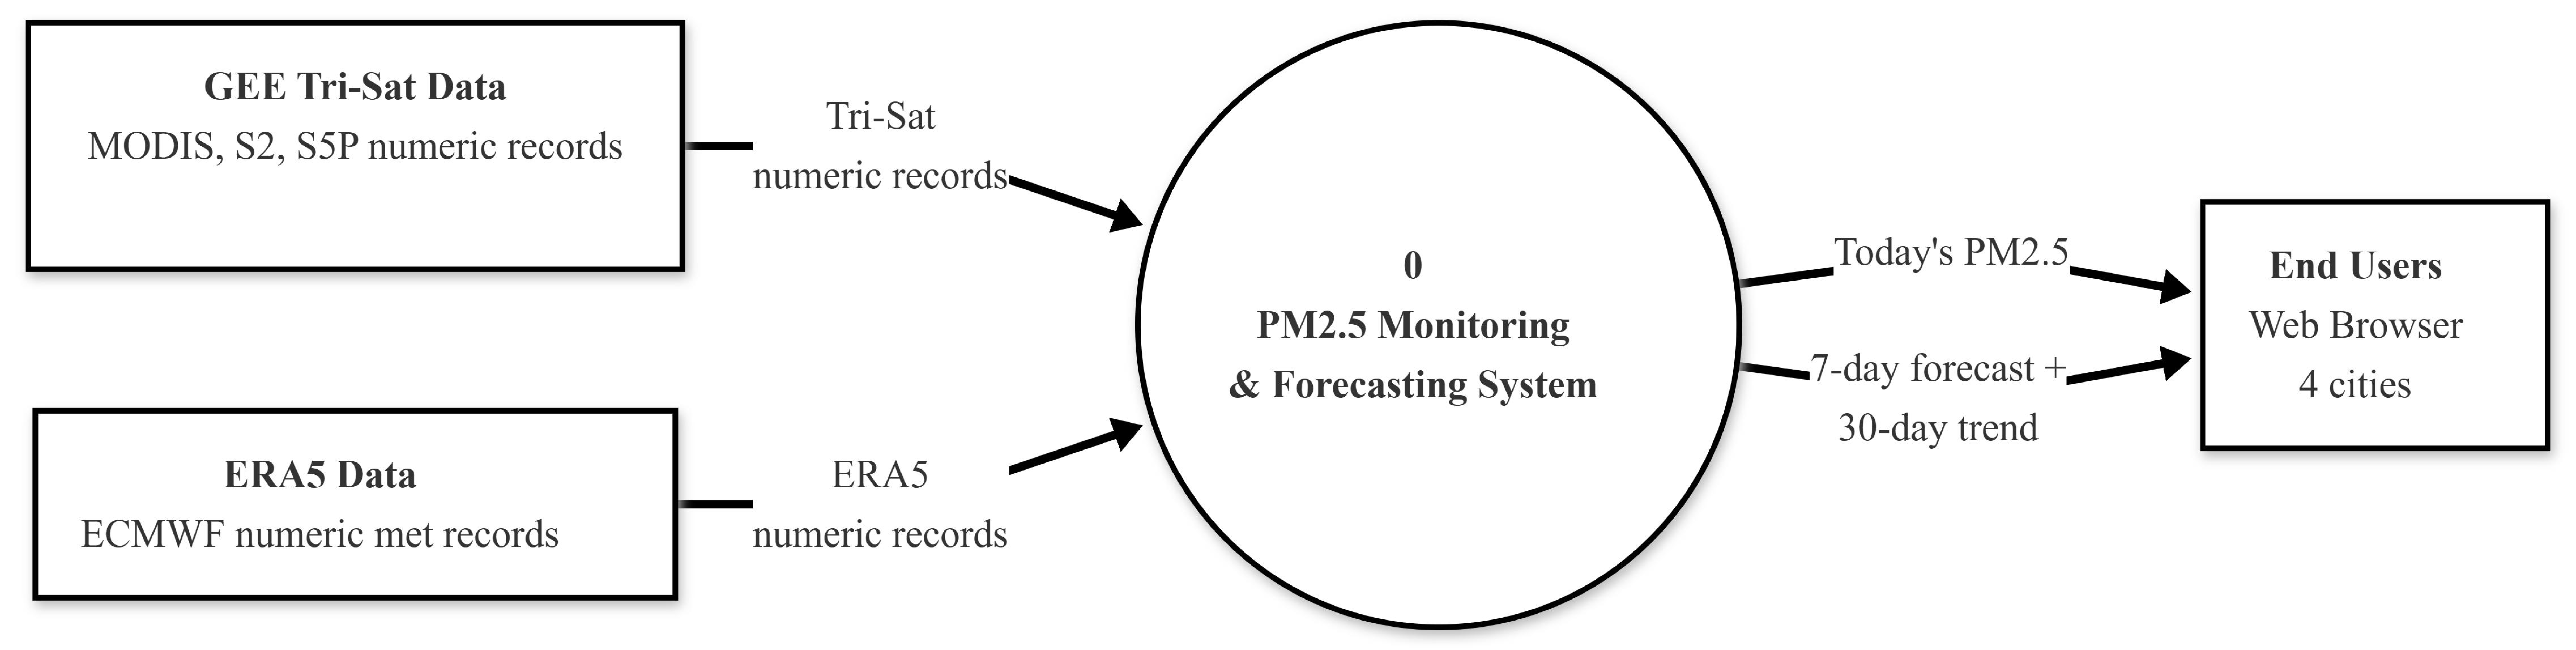
\includegraphics[width=0.8\textwidth]{pdfs/dfd0.pdf}
    \caption{DFD - Level 0}
    \label{fig:dfd0}
\end{figure}


Figure~\ref{fig:dfd0} presents the Level 0 Data Flow Diagram of the PM$_{2.5}$ monitoring and forecasting system. The system is represented as a single process interacting with three external entities: satellite data sources via Google Earth Engine, ERA5 meteorological reanalysis, and end users who access predictions and forecasts.


% ============================================================
\subsection{Level 1 DFD}
\label{subsec:dfd1}
% ============================================================
Figure~\ref{fig:dfd1} decomposes the system into six main processes, three data stores, and two external entities. It illustrates the flow of satellite and meteorological data through successive stages of preprocessing, feature extraction, PM$_{2.5}$ prediction, and LSTM-based forecasting. The diagram highlights how processed information is stored, combined with historical records, and ultimately delivered to end users through the web interface. This representation provides a clear overview of the system's data management and processing logic while abstracting away detailed algorithmic operations.



\begin{figure}[H]
    \centering
    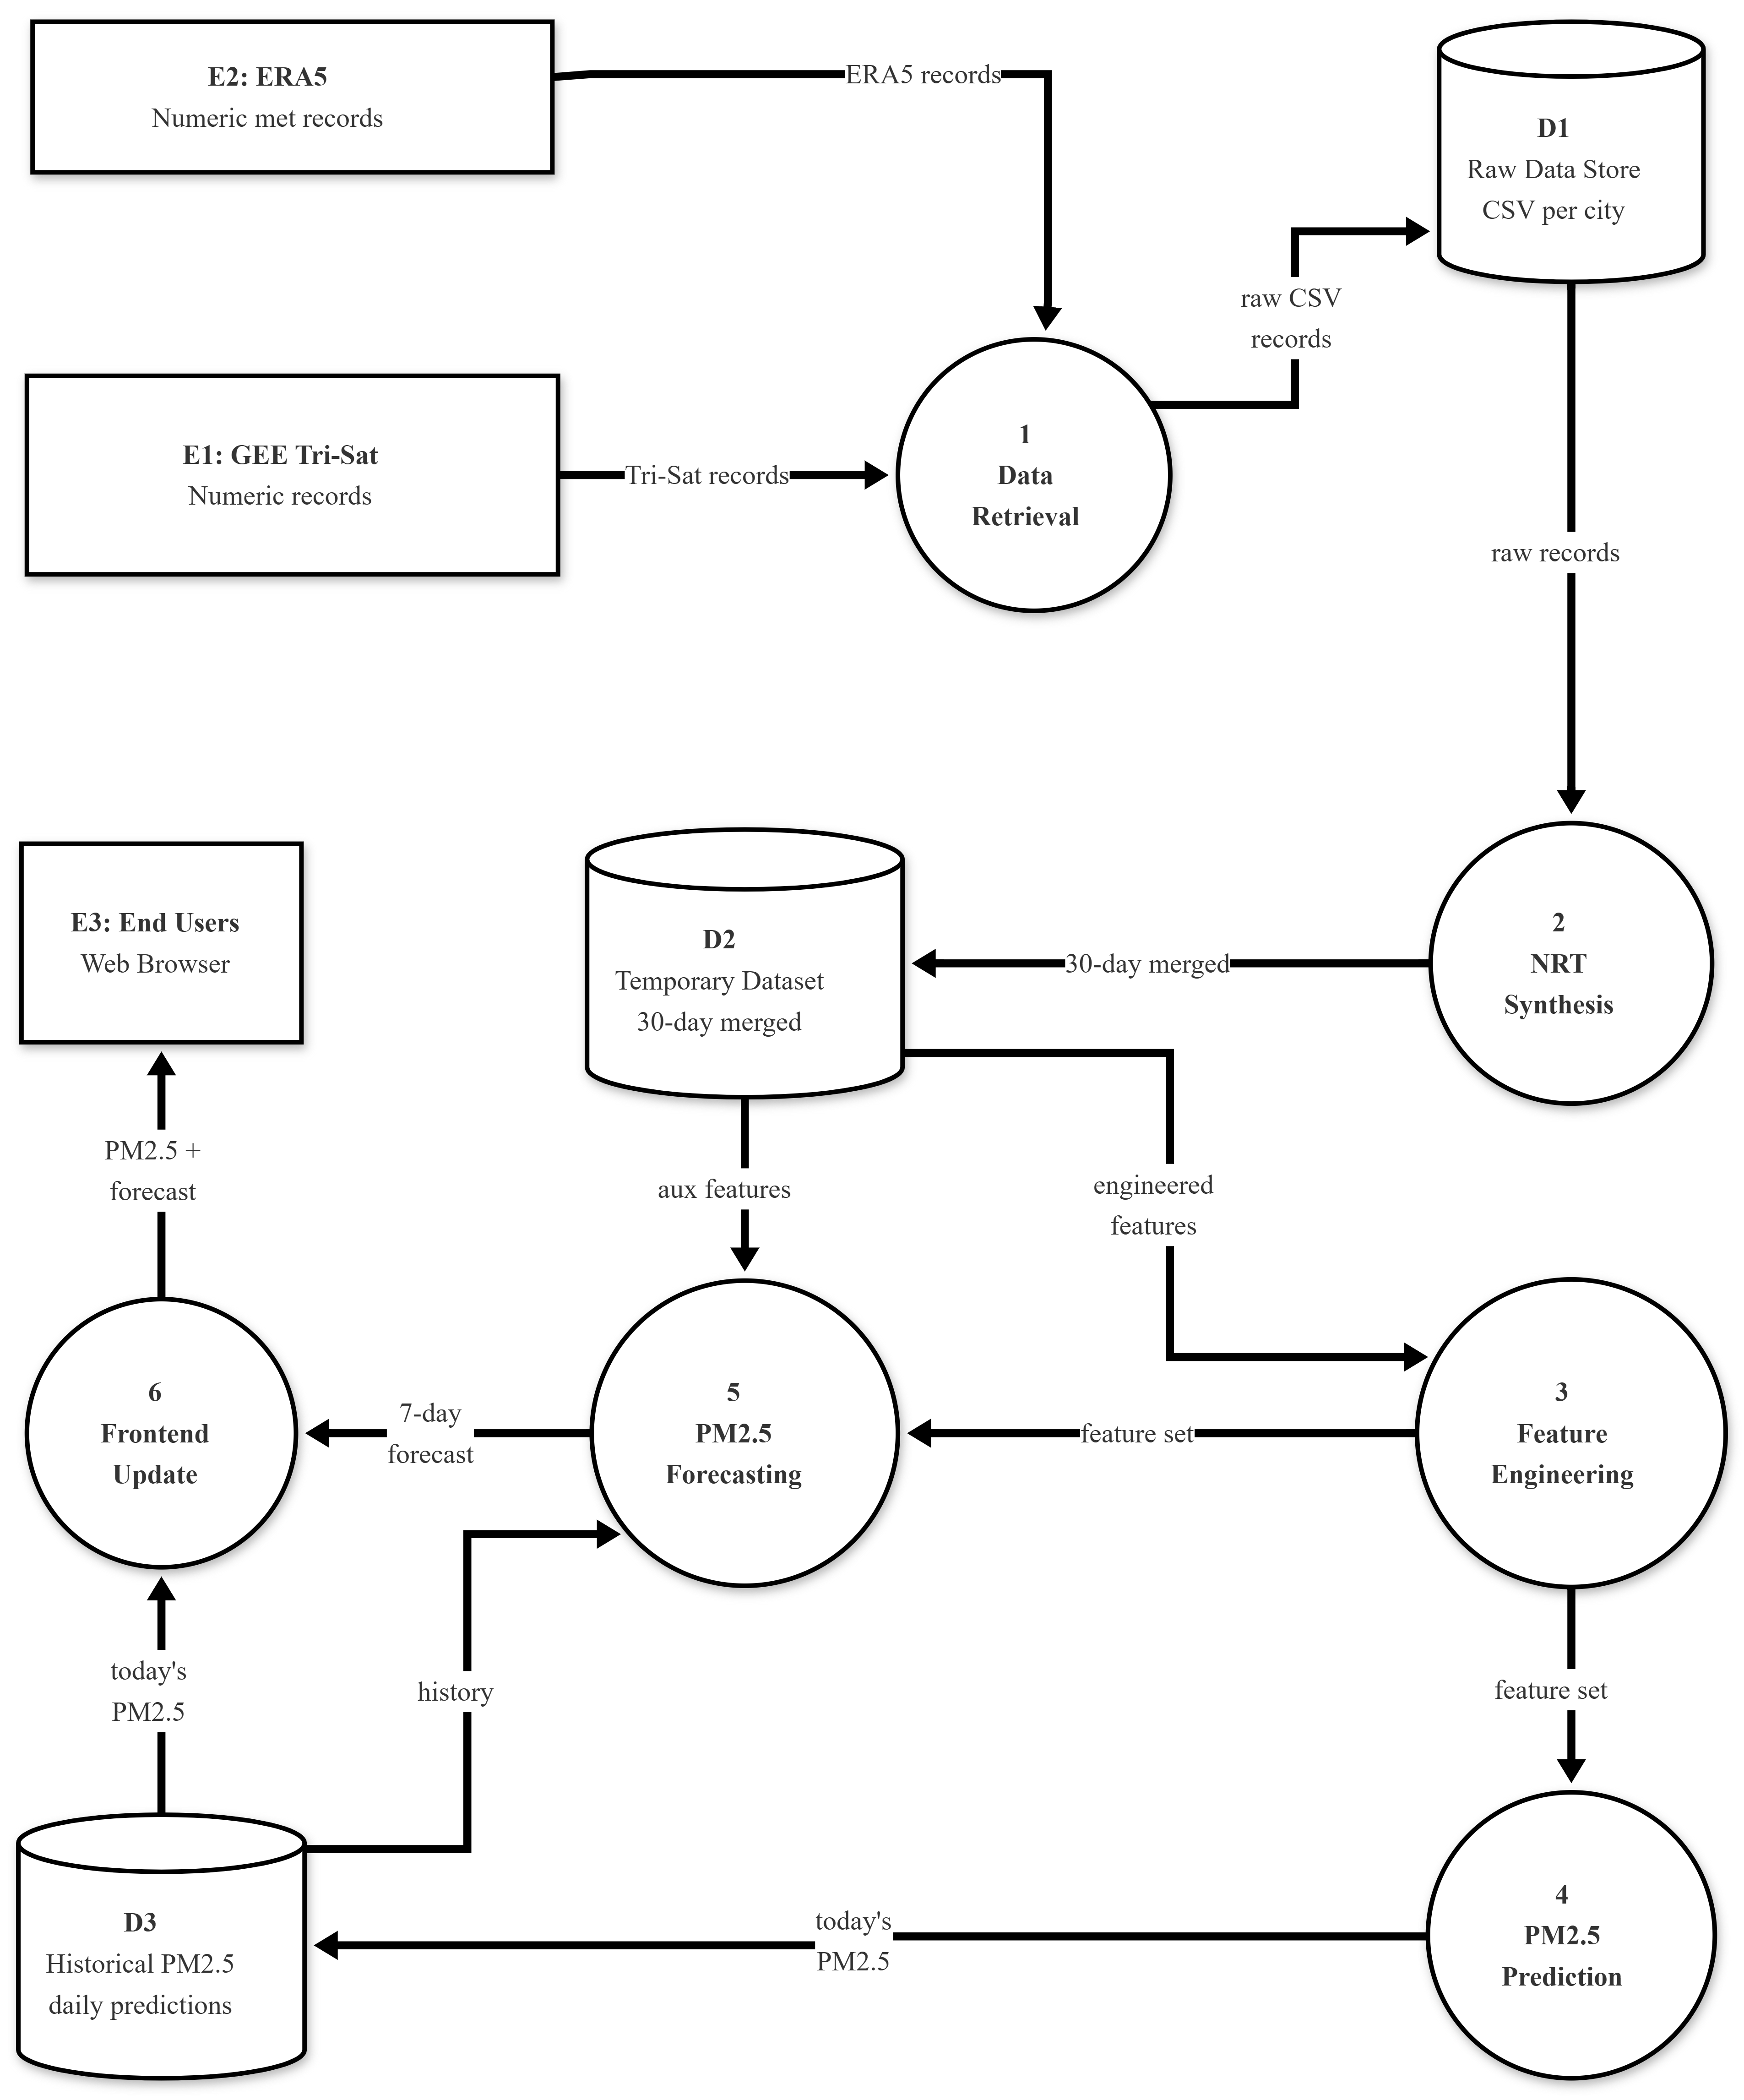
\includegraphics[width=0.8\textwidth]{Images/dfd1.png}
    \caption{{DFD - Level 1}
}
    \label{fig:dfd1}
\end{figure}




% ============================================================
\subsection{Level 2 DFDs}
\label{subsec:dfd2}
% ============================================================
The subsections below present the Level 2 Data Flow Diagrams for each of the six primary processes identified at Level 1. Each Level 2 DFD breaks down a single high-level process into its constituent sub-processes, showing how data flows internally, how it interacts with data stores, and how it connects with other modules. This detailed decomposition helps clarify the internal workings of the system and illustrates how raw inputs are transformed into processed outputs and forecasts.


% ---- Process 1 ----
\subsubsection{DFD Level 2.1}
\label{subsubsec:dfd2_1}

\begin{figure}[H]
    \centering
    \includegraphics[width=\textwidth]{pdfs/dfd2.1.pdf}
    \caption{DFD - Level 2.1: Data Retrieval Module}
    \label{fig:dfd2_1}
\end{figure}

Figure~\ref{fig:dfd2_1} shows the Data Retrieval Module (P1) broken into four steps. First, the system queries GEE to get numeric data from the Tri-Sat products for the target city and dates. Second, it retrieves ERA5 meteorological data. Third, a look-back check identifies any missing historical records and fetches them as needed. Finally, the retrieved data is validated and appended to D1, ensuring the raw data store keeps a complete and chronological record.



% ---- Process 2 ----
\subsubsection{DFD Level 2.2}
\label{subsubsec:dfd2_2}

\begin{figure}[H]
    \centering
    \includegraphics[width=\textwidth]{pdfs/dfd2.2.pdf}
    \caption{DFD - Level 2.2: NRT Synthesis Module}
    \label{fig:dfd2_2}
\end{figure}

Figure 6.4 shows the Level 2 DFD of the NRT Synthesis Module (P2), which fills temporal gaps in all input data. The most recent 45 days of ERA5 records are extracted from D1, and an internal LSTM predicts any missing values. Tri-Sat observations are checked, and missing values are estimated using city-specific regression models. All raw and predicted data are merged into D2, producing a consistent 30-day dataset for downstream feature engineering and PM$_{2.5}$ prediction.

% ---- Process 3 ----
\subsubsection{DFD Level 2.3}
\label{subsubsec:dfd2_3}

\begin{figure}[H]
    \centering
    \includegraphics[width=0.8\textwidth]{pdfs/dfd2.3.pdf}
    \caption{DFD - Level 2.3: Feature Engineering Module}
    \label{fig:dfd2_3}
\end{figure}

Figure~\ref{fig:dfd2_3} shows the Level 2 DFD of the Feature Engineering Module (P3), which transforms D2 into a structured feature matrix for machine learning. Sensor streams are aligned to a common daily grid, and satellite indices (NDVI, AOD ratios, MODIS fire counts, TROPOMI columns) are computed. Meteorological features from ERA5, temporal lag features, and rolling statistics are generated. Continuous variables are normalized, and calendar features are cyclically encoded. The same process is applied for the Forecasting Model (P5) to ensure consistent inputs.


% ---- Process 4 ----
\subsubsection{DFD Level 2.4}
\label{subsubsec:dfd2_4}

\begin{figure}[H]
    \centering
    \includegraphics[width=\textwidth]{pdfs/dfd2.4.pdf}
    \caption{DFD - Level 2.4: Ensemble PM2.5 Prediction Model}
    \label{fig:dfd2_4}
\end{figure}

Figure~\ref{fig:dfd2_4} shows the Level 2 DFD of the Ensemble PM2.5 Prediction Model (P4), which produces daily PM2.5 estimates from the engineered features. The model combines four tree-based learners: Random Forest, XGBoost, LightGBM, and CatBoost, each trained on historical satellite and ERA5 data with ground-truth PM2.5 values. Their predictions are then combined using a stacking meta-learner to produce the final estimate, which is stored in D3 and sent to the Frontend Update module (P6) for display.
.

% ---- Process 5 ----
\subsubsection{DFD Level 2.5}
\label{subsubsec:dfd2_5}

\begin{figure}[H]
    \centering
    \includegraphics[width=\textwidth]{pdfs/dfd2.5.pdf}
    \caption{DFD - Level 2.5: LSTM PM2.5 Forecasting Model}
    \label{fig:dfd2_5}
\end{figure}

Figure~\ref{fig:dfd2_5} shows the LSTM Forecasting Model (P5), which generates a 7-day PM2.5 forecast. It uses the previous 30–45 days of predictions from D3 along with corresponding features from D2. The same Feature Engineering Module (P3) ensures consistent input formatting. The data is reshaped into a tensor for the stacked LSTM network, which outputs PM2.5 values for the next seven days. Models are city-specific to capture local pollution patterns, and the forecasts are sent to the Frontend Update module (P6) for display.



% ---- Process 6 ----
\subsubsection{DFD Level 2.6}
\label{subsubsec:dfd2_6}

\begin{figure}[H]
    \centering
    \includegraphics[width=0.85\textwidth]{pdfs/dfd2.6.pdf}
    \caption{DFD - Level 2.6: Frontend Update}
    \label{fig:dfd2_6}
\end{figure}

Figure~\ref{fig:dfd2_6} shows the Level 2 DFD of the LSTM Forecasting Model (P5), which produces a 7-day PM2.5 forecast. It takes the last 30–45 days of predictions from D3 along with matching features from D2. The Feature Engineering Module (P3) is applied to ensure consistent inputs. The data is reshaped for the stacked LSTM network, which outputs PM2.5 values for the next seven days. City-specific models capture local pollution patterns, and the forecasts are sent to the Frontend Update module (P6) for display.

\section{Methodological Framework}

The proposed system follows a modular machine learning framework consisting of data retrieval, preprocessing, gap-filling, prediction, and forecasting stages. All predictive components were developed using supervised learning techniques trained in historical satellite ,meteorological, and ground observation datasets.

\begin{figure}[H]
    \centering
    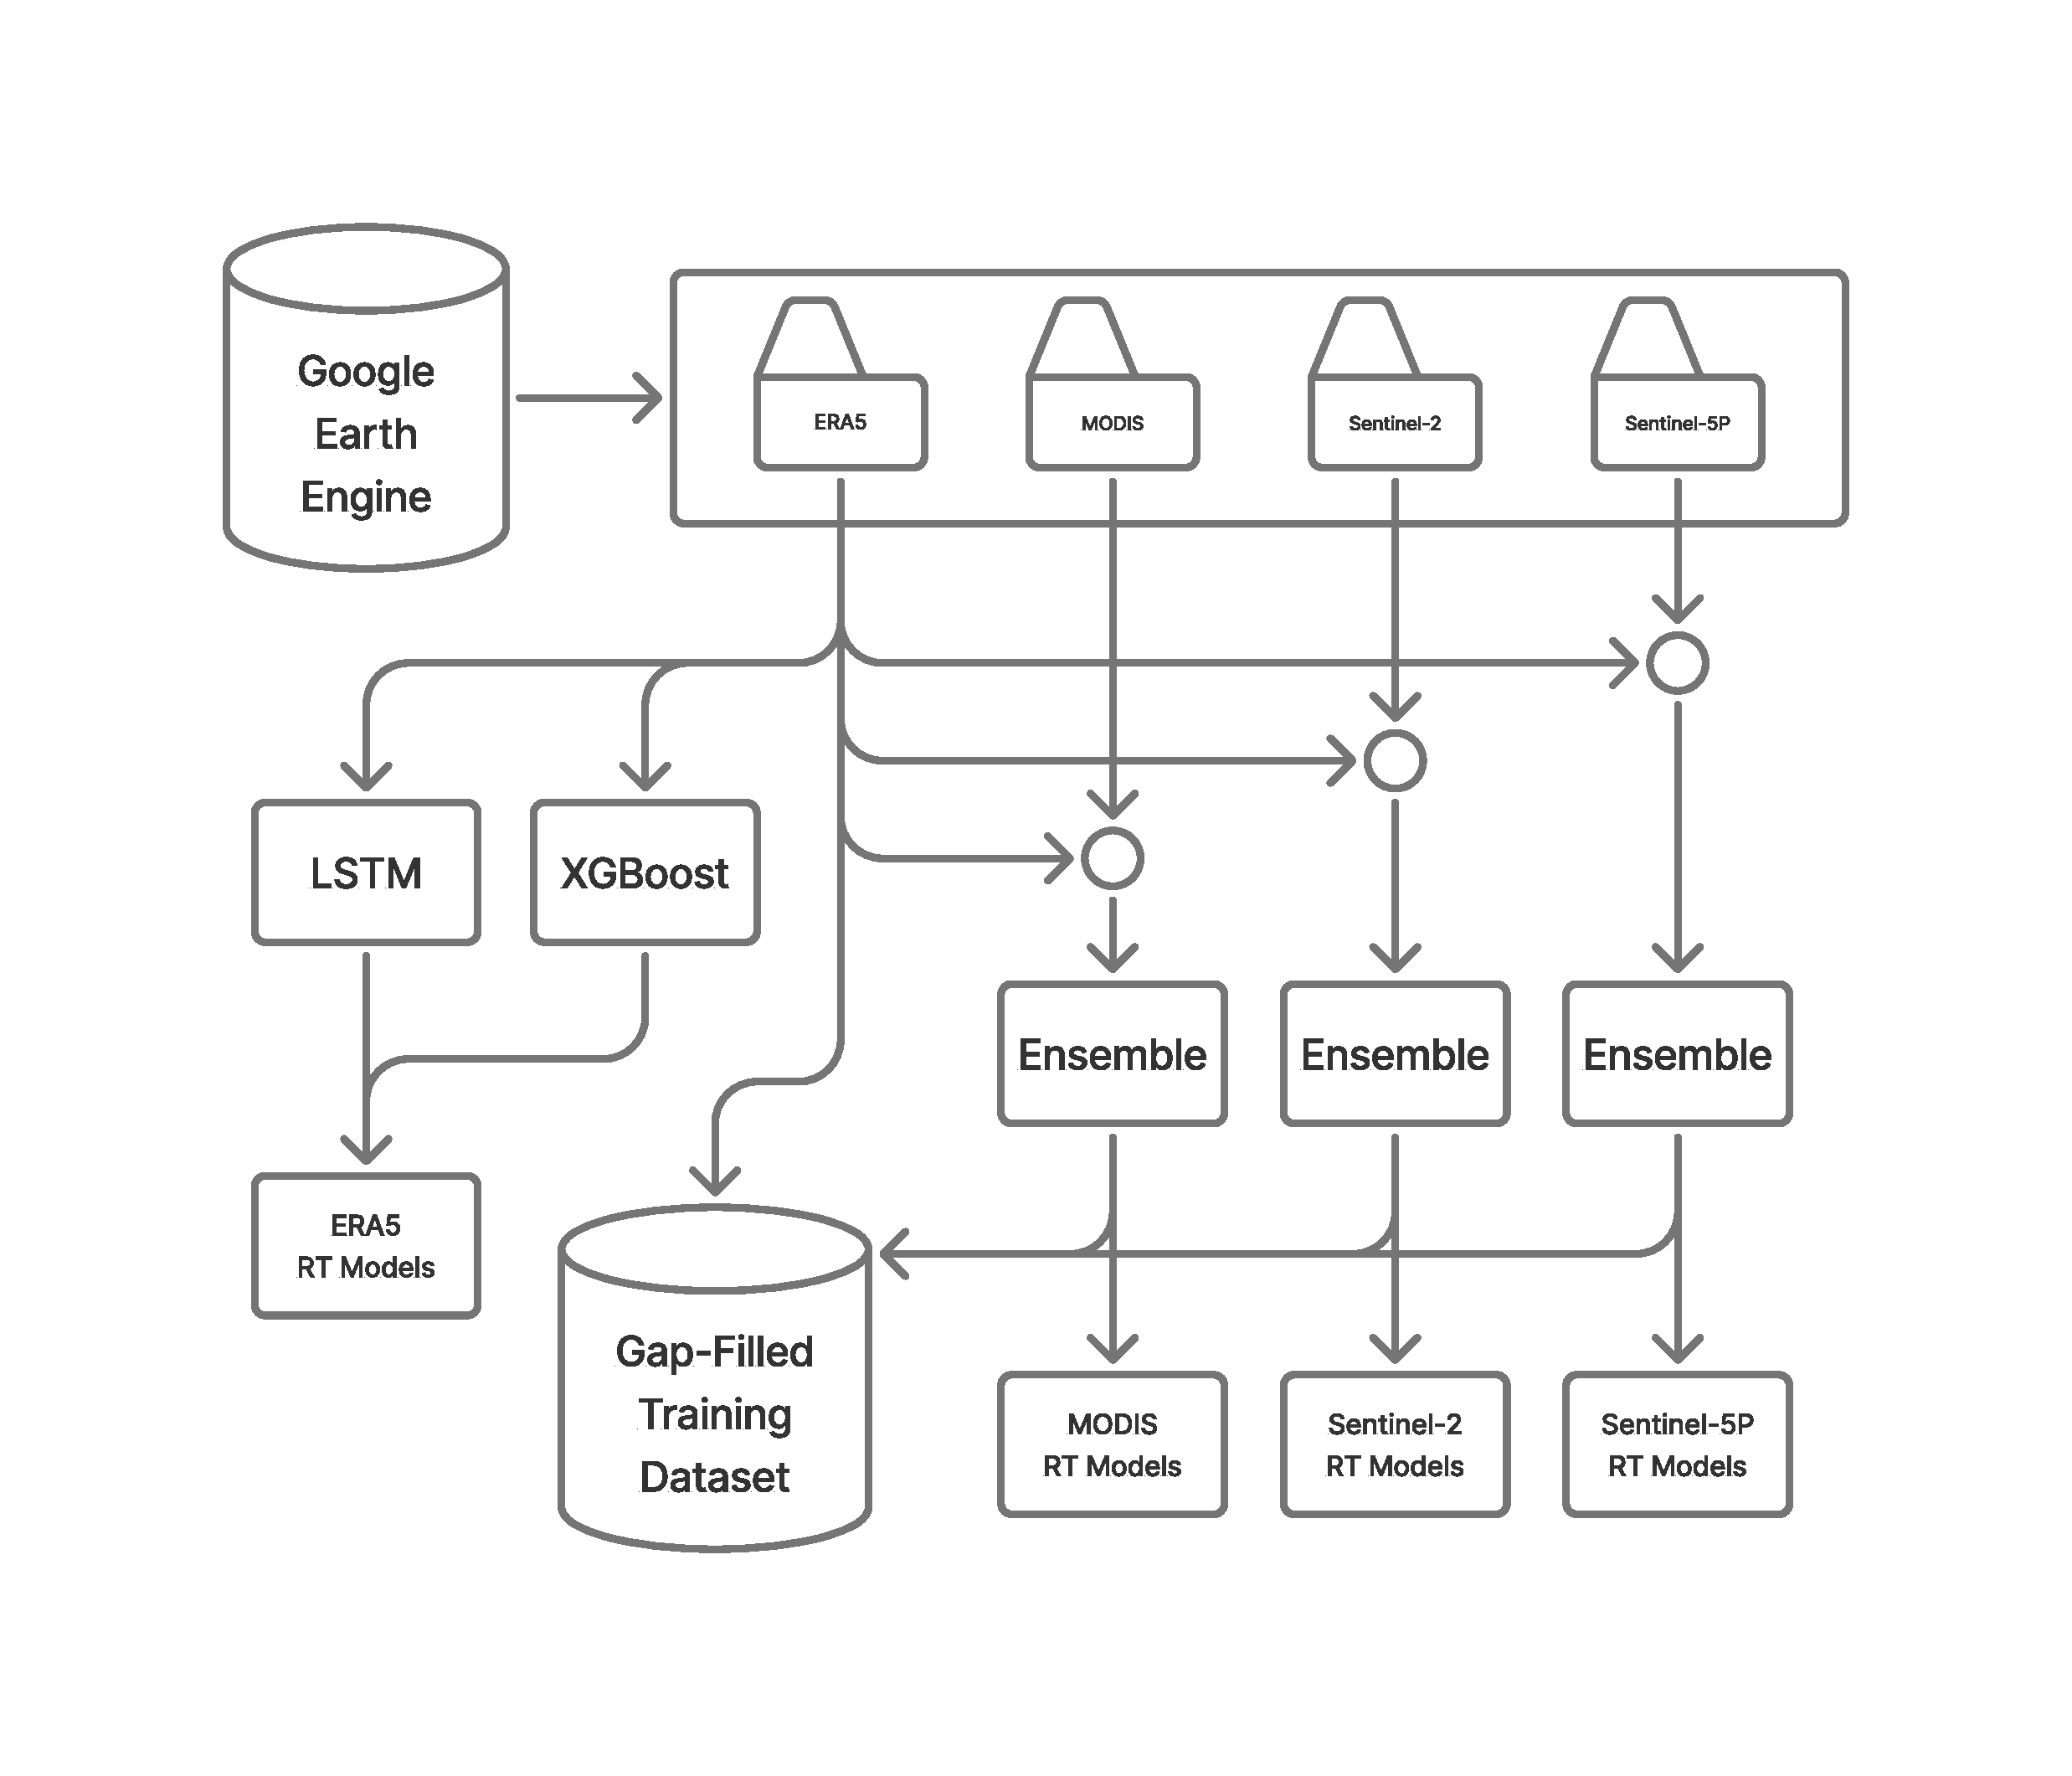
\includegraphics[width=0.65\linewidth]{pdfs/method1.pdf}
    \caption{Satellite gap-filling and real time model pipelining}
    \label{fig:placeholder}
\end{figure}
Time-series aware validation strategies were adopted to prevent data leakage. Hyperparameter optimization was performed using automated search methods, and early stopping was applied to reduce overfitting. Where atmospheric dynamics differed significantly across cities, city-specific models were trained to capture localized behavior.
Gap-filling models were developed to handle missing satellite observations caused by cloud cover and data latency. Meteorological forecasting models were constructed to overcome ERA5 release delays, ensuring real-time operability. These trained models were later integrated into the deployment pipeline described in subsequent sections.

\subsection{Model Validation and Testing Strategy}

To ensure realistic deployment performance, different validation strategies were adopted depending on the model type.

For real-time operational models, including the ERA5 meteorological forecasting and satellite gap-filling components, chronological validation was employed. Training was conducted on historical data up to a defined cutoff date, while evaluation was performed on subsequent unseen time periods. This approach simulates real-world deployment conditions and prevents temporal data leakage.

For the PM$_{2.5}$ prediction and 7-day forecasting models, site-specific validation against ground truth monitoring stations was performed. Each city's model was evaluated using locally observed PM$_{2.5}$ measurements to ensure that spatially varying atmospheric dynamics were accurately captured.

These validation strategies were designed to reflect both temporal generalization and spatial reliability in operational conditions.

% =====================================================================

\newpage

\chapter{Task Accomplished}
\section{Data Collection and Integration}

A major portion of the mid-term phase was dedicated to the collection, preprocessing, and integration of multi-source datasets required for PM$_{2.5}$ prediction. Satellite-based atmospheric observations, meteorological reanalysis data, and ground-based air quality measurements were systematically retrieved, processed, and aligned to form a unified dataset suitable for machine learning and time-series modeling.

\subsection{ERA5 Reanalysis Data}

Meteorological and land surface variables were collected from the ERA5 reanalysis product to capture atmospheric dynamics influencing particulate matter concentration. The retrieved parameters include air temperature, dew point temperature, relative humidity, precipitation, surface pressure, wind speed, wind direction, surface water content, soil water content, evaporation, solar radiation, thermal radiation, leaf area indices, and boundary layer height.

Several variables, such as relative humidity and wind characteristics, were derived from primary ERA5 parameters to ensure physical consistency. All ERA5 variables were aggregated to daily temporal resolution and spatially averaged within an approximate 5.5~km radius buffer to maintain compatibility with satellite-derived datasets. The ERA5 data provide long-term historical coverage beginning from January 2000, enabling temporal continuity across multiple satellite missions.

\subsection{MODIS Aerosol Data}

Aerosol Optical Depth (AOD) at 550~nm was collected from MODIS products to represent columnar aerosol loading, which is strongly associated with surface-level PM$_{2.5}$. MODIS data were processed at daily temporal resolution and spatially averaged using circular buffers of 5000~m and 600~m radius.

Quality assurance flags were applied to remove low-confidence retrievals and cloud-contaminated pixels before aggregation. The processed MODIS AOD data offer long-term aerosol information starting from February 2000 and serve as a key proxy variable linking satellite observations to ground-level particulate pollution.

\subsection{Sentinel-2 Optical and Atmospheric Data}

Sentinel-2 data were collected to extract high-resolution optical and atmospheric information relevant to surface and near-surface pollution characteristics. Multiple spectral bands spanning the visible, near-infrared, and shortwave infrared regions were retrieved, along with atmospheric products such as Aerosol Optical Thickness and Water Vapor Product.

All Sentinel-2 data were aggregated to daily resolution using fixed spatial buffers of 5000~m and 600~m radius. Cloud masking and quality filtering were applied prior to aggregation to reduce noise and ensure reliability. The inclusion of Sentinel-2 features enhances the spatial detail of the dataset and supports improved representation of land surface and atmospheric conditions from 2017 onward.

\subsection{Sentinel-5P Trace Gas Observations}

Trace gas concentrations and absorbing aerosol indices were obtained from Sentinel-5P to capture atmospheric composition associated with emission sources and secondary aerosol formation. The extracted variables include nitrogen dioxide, sulfur dioxide, carbon monoxide, ozone, formaldehyde, and aerosol index.

These variables were processed to daily aggregates and spatially averaged within circular buffers of 5000~m and 600~m radius to maintain consistency across satellite sources. Sentinel-5P data provide chemically relevant indicators of anthropogenic and photochemical processes affecting PM$_{2.5}$ levels, with coverage available from mid-2018.

\subsection{Ground-Based PM$_{2.5}$ Measurements}

Daily average PM$_{2.5}$ concentrations were collected from the OpenAQ platform to serve as ground truth observations. These measurements were obtained from regulatory and low-cost monitoring stations and represent point-based sensor data.

The OpenAQ PM$_{2.5}$ values were temporally aligned with satellite and reanalysis datasets. Due to varying sensor availability, temporal coverage differs by location; however, all available observations were retained to maximize training and evaluation samples.

\subsection{Temporal Feature Engineering and Dataset Alignment}

To account for seasonal and cyclic variations in air pollution, sine and cosine transformations of the day of the year were computed and added as temporal features. These features enable the models to learn periodic patterns without introducing artificial discontinuities.

Finally, all datasets were synchronized to a common daily temporal resolution and integrated into a single structured dataset. PM$_{2.5}$ was designated as the target variable, while all satellite-, reanalysis-, and time-derived parameters were treated as input features. This integrated dataset forms the foundation for subsequent ensemble learning and LSTM-based model development.

\section{ERA5 Forecasting for Real-Time Deployment}

ERA5 provides a comprehensive set of meteorological variables with full spatial coverage; however, its operational release is delayed by 7--8 days, which prevents direct real-time use for PM$_{2.5}$ prediction. For instance, if today is Day 8, the most recent ERA5 data available corresponds to Day 1. To address this latency, we implemented a forecasting framework for deployment sites to ensure a continuous, gap-free set of meteorological features.

The forecasting framework combines two machine learning approaches:

\begin{enumerate}
    \item \textbf{LSTM with Attention:} Used to predict continuous variables such as temperature, humidity, wind speed, boundary layer height, and radiation fluxes. The model incorporates 45-day historical sequences to capture temporal dependencies and seasonal patterns. The attention mechanism allows the model to weigh critical time steps, improving prediction accuracy for variables with non-linear temporal trends.
    
    \item \textbf{XGBoost Rain Classifier:} Precipitation is predicted using a two-step approach. First, XGBoost classifies each day as rain or no-rain. Only when rain is predicted does the LSTM generate a precipitation amount; otherwise, the daily value is set to zero. This strategy effectively handles the intermittent and sparse nature of rainfall.
\end{enumerate}

The LSTM forecaster was trained using data from four deployment sites in Nepal: Kathmandu, Pokhara, Chitwan, and Birgunj. Hyperparameters were optimized via Bayesian search using Optuna, resulting in a hidden size of 512, three stacked LSTM layers, a sequence length of 45 days, and dropout of 0.15 to prevent overfitting. The attention mechanism was enabled to capture long-range dependencies effectively.

\begin{table}[H]
\centering
\caption{Optimized Hyperparameters of the LSTM Forecaster}
\vspace{.5cm}
\begin{tabular}{|l|l|}
\hline
\textbf{Hyperparameter} & \textbf{Value} \\
\hline
Hidden size & 512 \\
\hline
Number of layers & 3 \\
\hline
Sequence length & 45 days \\
\hline
Dropout & 0.15 \\
\hline
Attention mechanism & Enabled \\
\hline
\end{tabular}
\end{table}

For training sites with complete historical ERA5 data, forecasting is unnecessary and observed values are used directly. For deployment sites, the hybrid system ensures real-time availability of all meteorological features, supporting daily PM$_{2.5}$ prediction without gaps. Across 16 ERA5 variables, the framework demonstrates robust predictive performance, effectively bridging the operational latency of ERA5 while maintaining high accuracy.
\subsection{Results}

\subsubsection{ERA5 Per-Variable Forecasting Performance}

Table~\ref{tab:era5_performance} presents the per-variable forecasting performance of the ERA5 forecaster across the four deployment sites. Variables with strong seasonal and temporal persistence, such as pressure, temperature, and leaf area index, achieve near-perfect prediction, whereas stochastic variables, particularly precipitation and surface runoff, show lower accuracy.

\begin{table}[h!]
\centering
\caption{Forecasting performance of ERA5 variables using LSTM across deployment sites.}
\vspace{.2cm}
\label{tab:era5_performance}
\begin{tabular}{|l|c|c|l|}
\hline
\textbf{Variable} & \textbf{$R^2$} & \textbf{Accuracy (\%)} & \textbf{Physical Interpretation} \\
\hline
press & 0.998 & 99.7 & Highly predictable \\
\hline
lei\_h & 0.999 & 98.9 & Seasonal cycle dominant \\
\hline
temp & 0.988 & 97.2 & Strong diurnal/seasonal cycles \\
\hline
dew & 0.986 & 90.8 & Tracks temperature with lag \\
\hline
lei\_l & 0.990 & 98.2 & Smooth vegetation phenology \\
\hline
t\_rad & 0.984 & 98.5 & Follows temperature closely \\
\hline
soil\_water & 0.977 & 95.5 & Slow-changing, high persistence \\
\hline
humi & 0.957 & 96.5 & Moderately variable \\
\hline
evapo & 0.949 & 90.2 & Depends on radiation and wind \\
\hline
blh & 0.944 & 88.5 & High day-to-day variability \\
\hline
wspeed & 0.934 & 98.5 & Chaotic short-term trends \\
\hline
so\_rad & 0.933 & 92.2 & Affected by clouds \\
\hline
preci & 0.931 & 72.5 & Stochastic, hardest to predict \\
\hline
surf\_water & 0.910 & 77.5 & Cascading errors from precipitation \\
\hline
wdir\_cos & 0.883 & 83.2 & Circular and noisy \\
\hline
wdir\_sin & 0.869 & 81.9 & Large sin/cos swings \\
\hline
\textbf{Average} & \textbf{0.952} & \textbf{91.3} & --- \\
\hline
\end{tabular}
\end{table}

\subsubsection{Precipitation Enhancement}

Due to the binary nature of rainfall, the LSTM forecaster alone struggles to predict precipitation accurately. Fig~\ref{rain_performance} shows the performance of the supplementary XGBoost rain classifier, which first predicts rain occurrence; the LSTM then estimates the rainfall amount for rain days.

\newpage

\begin{figure}[H] \centering 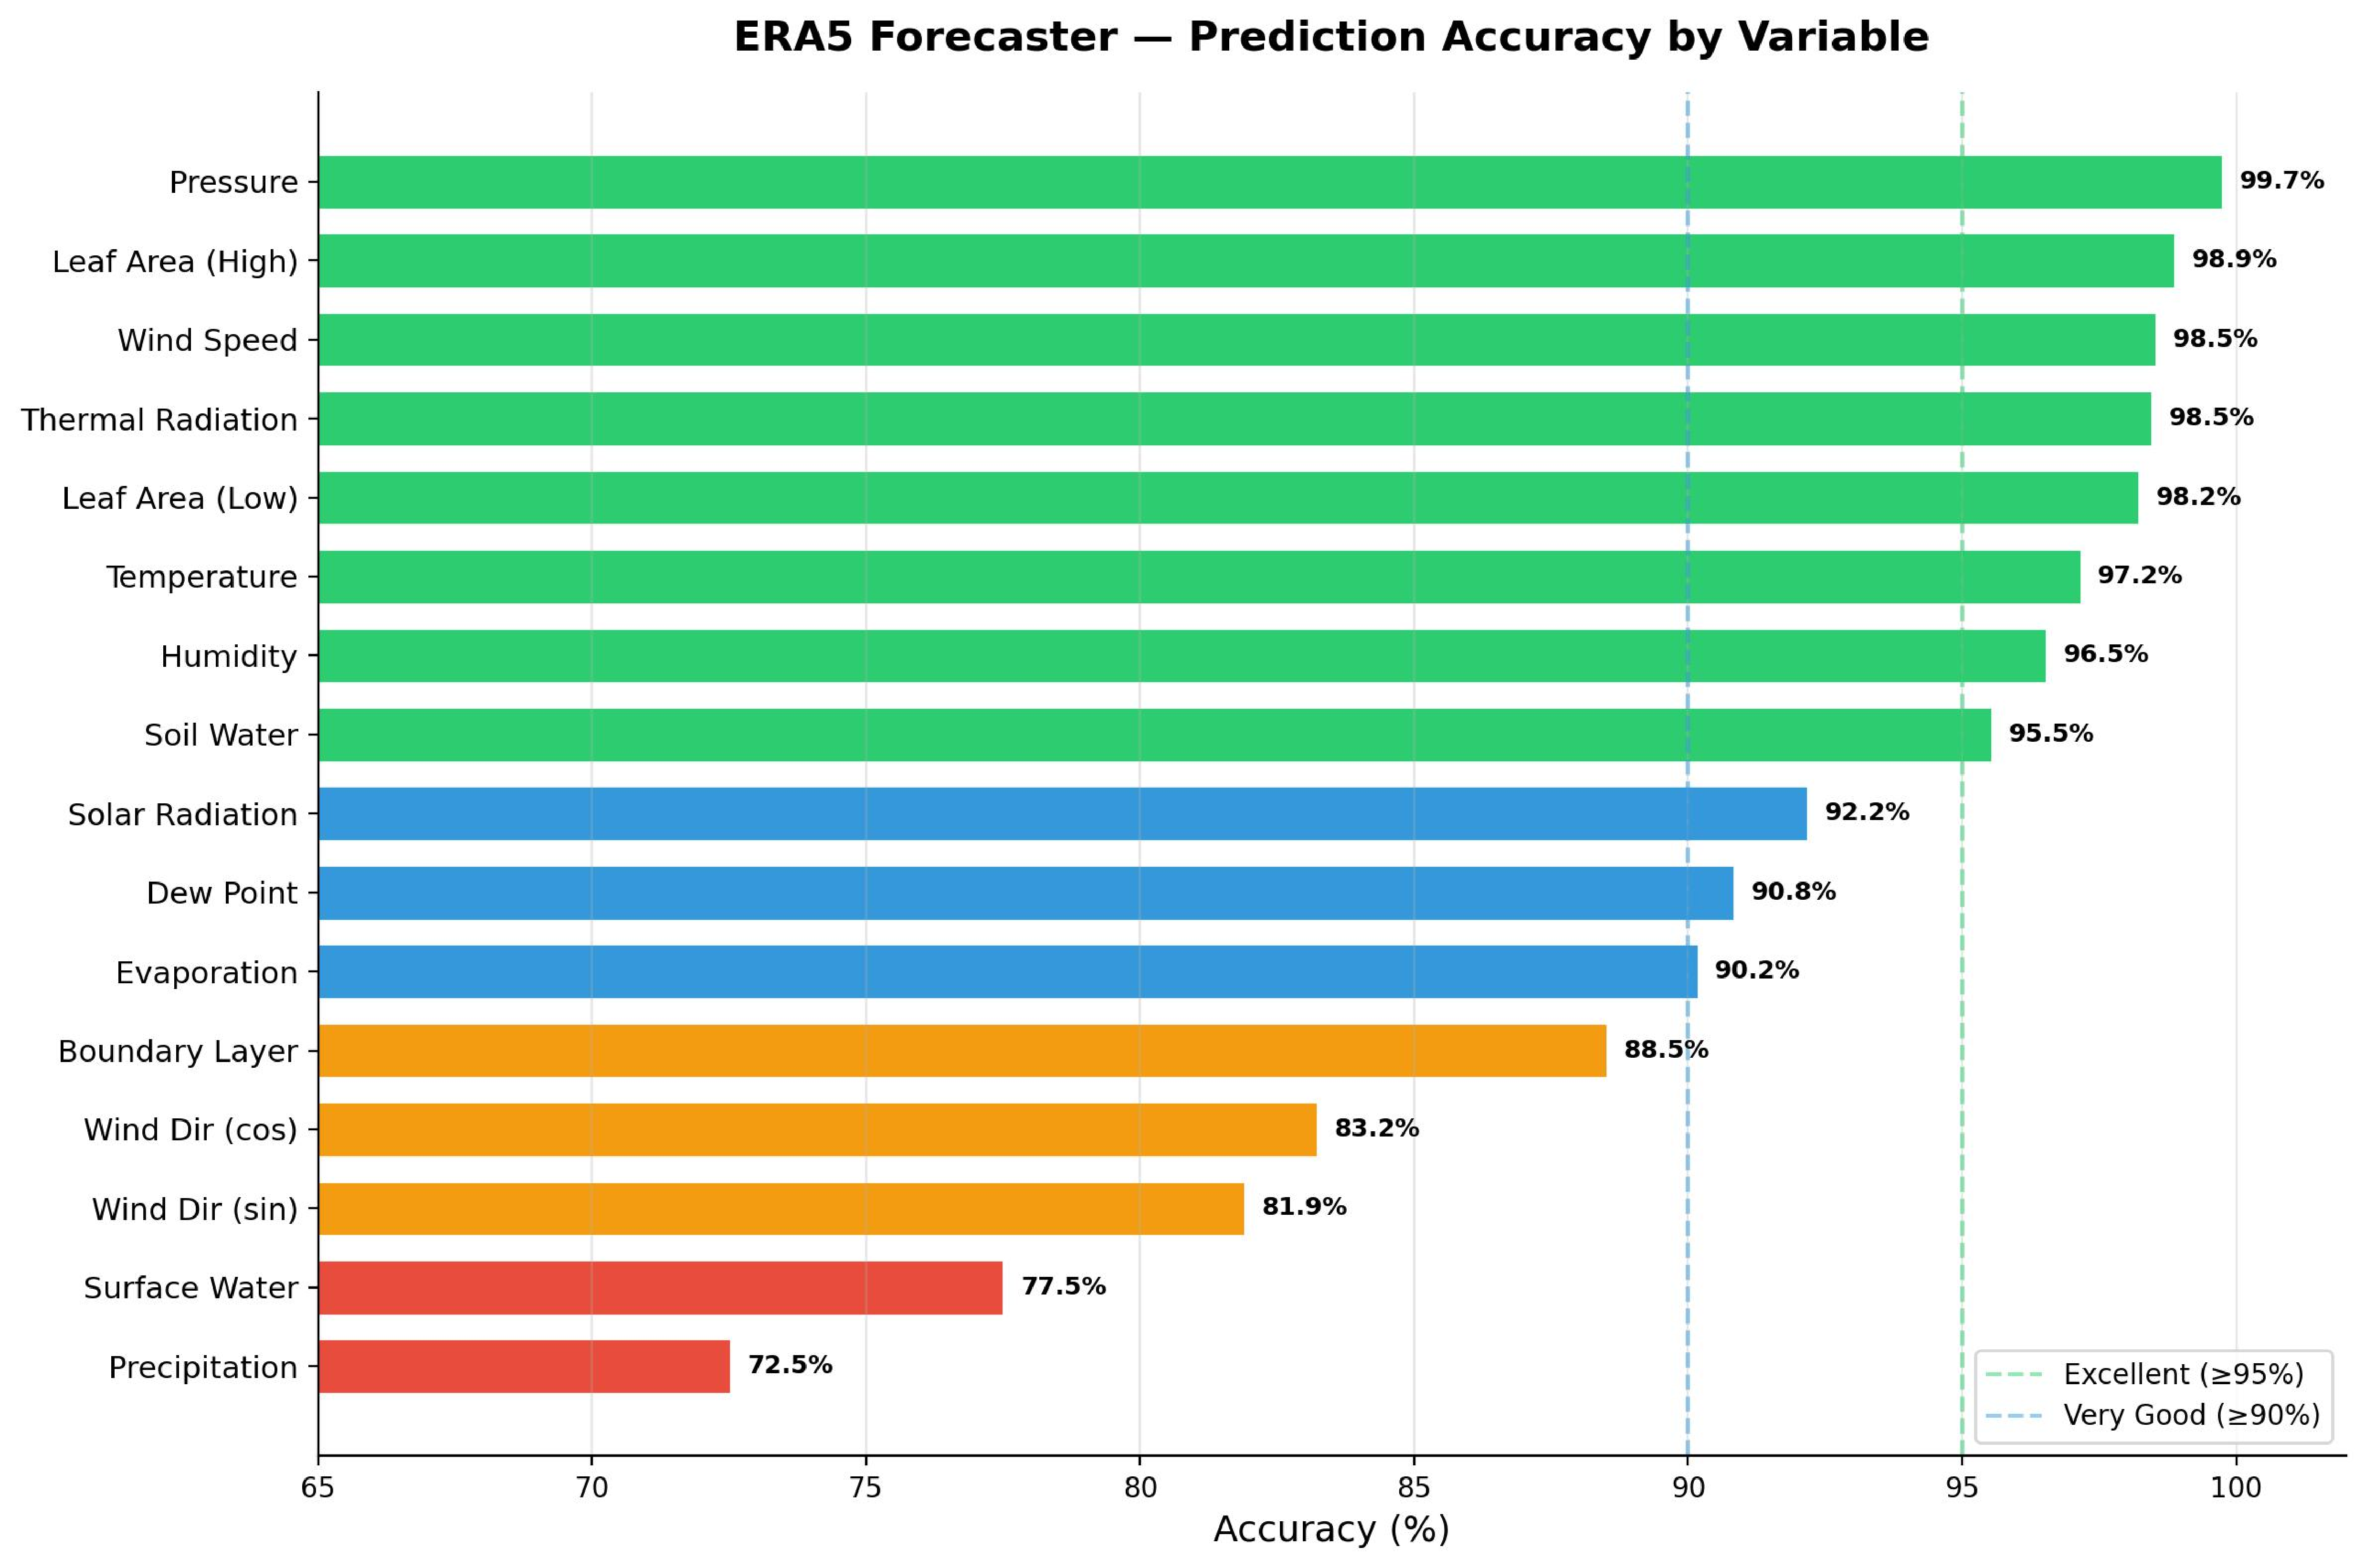
\includegraphics[width=1\linewidth]{pdfs/era5-acc.pdf} \caption{ERA-5 Forecaster Accuracy Chart} \label{fig:placeholder} \end{figure} \begin{figure}[H] \centering 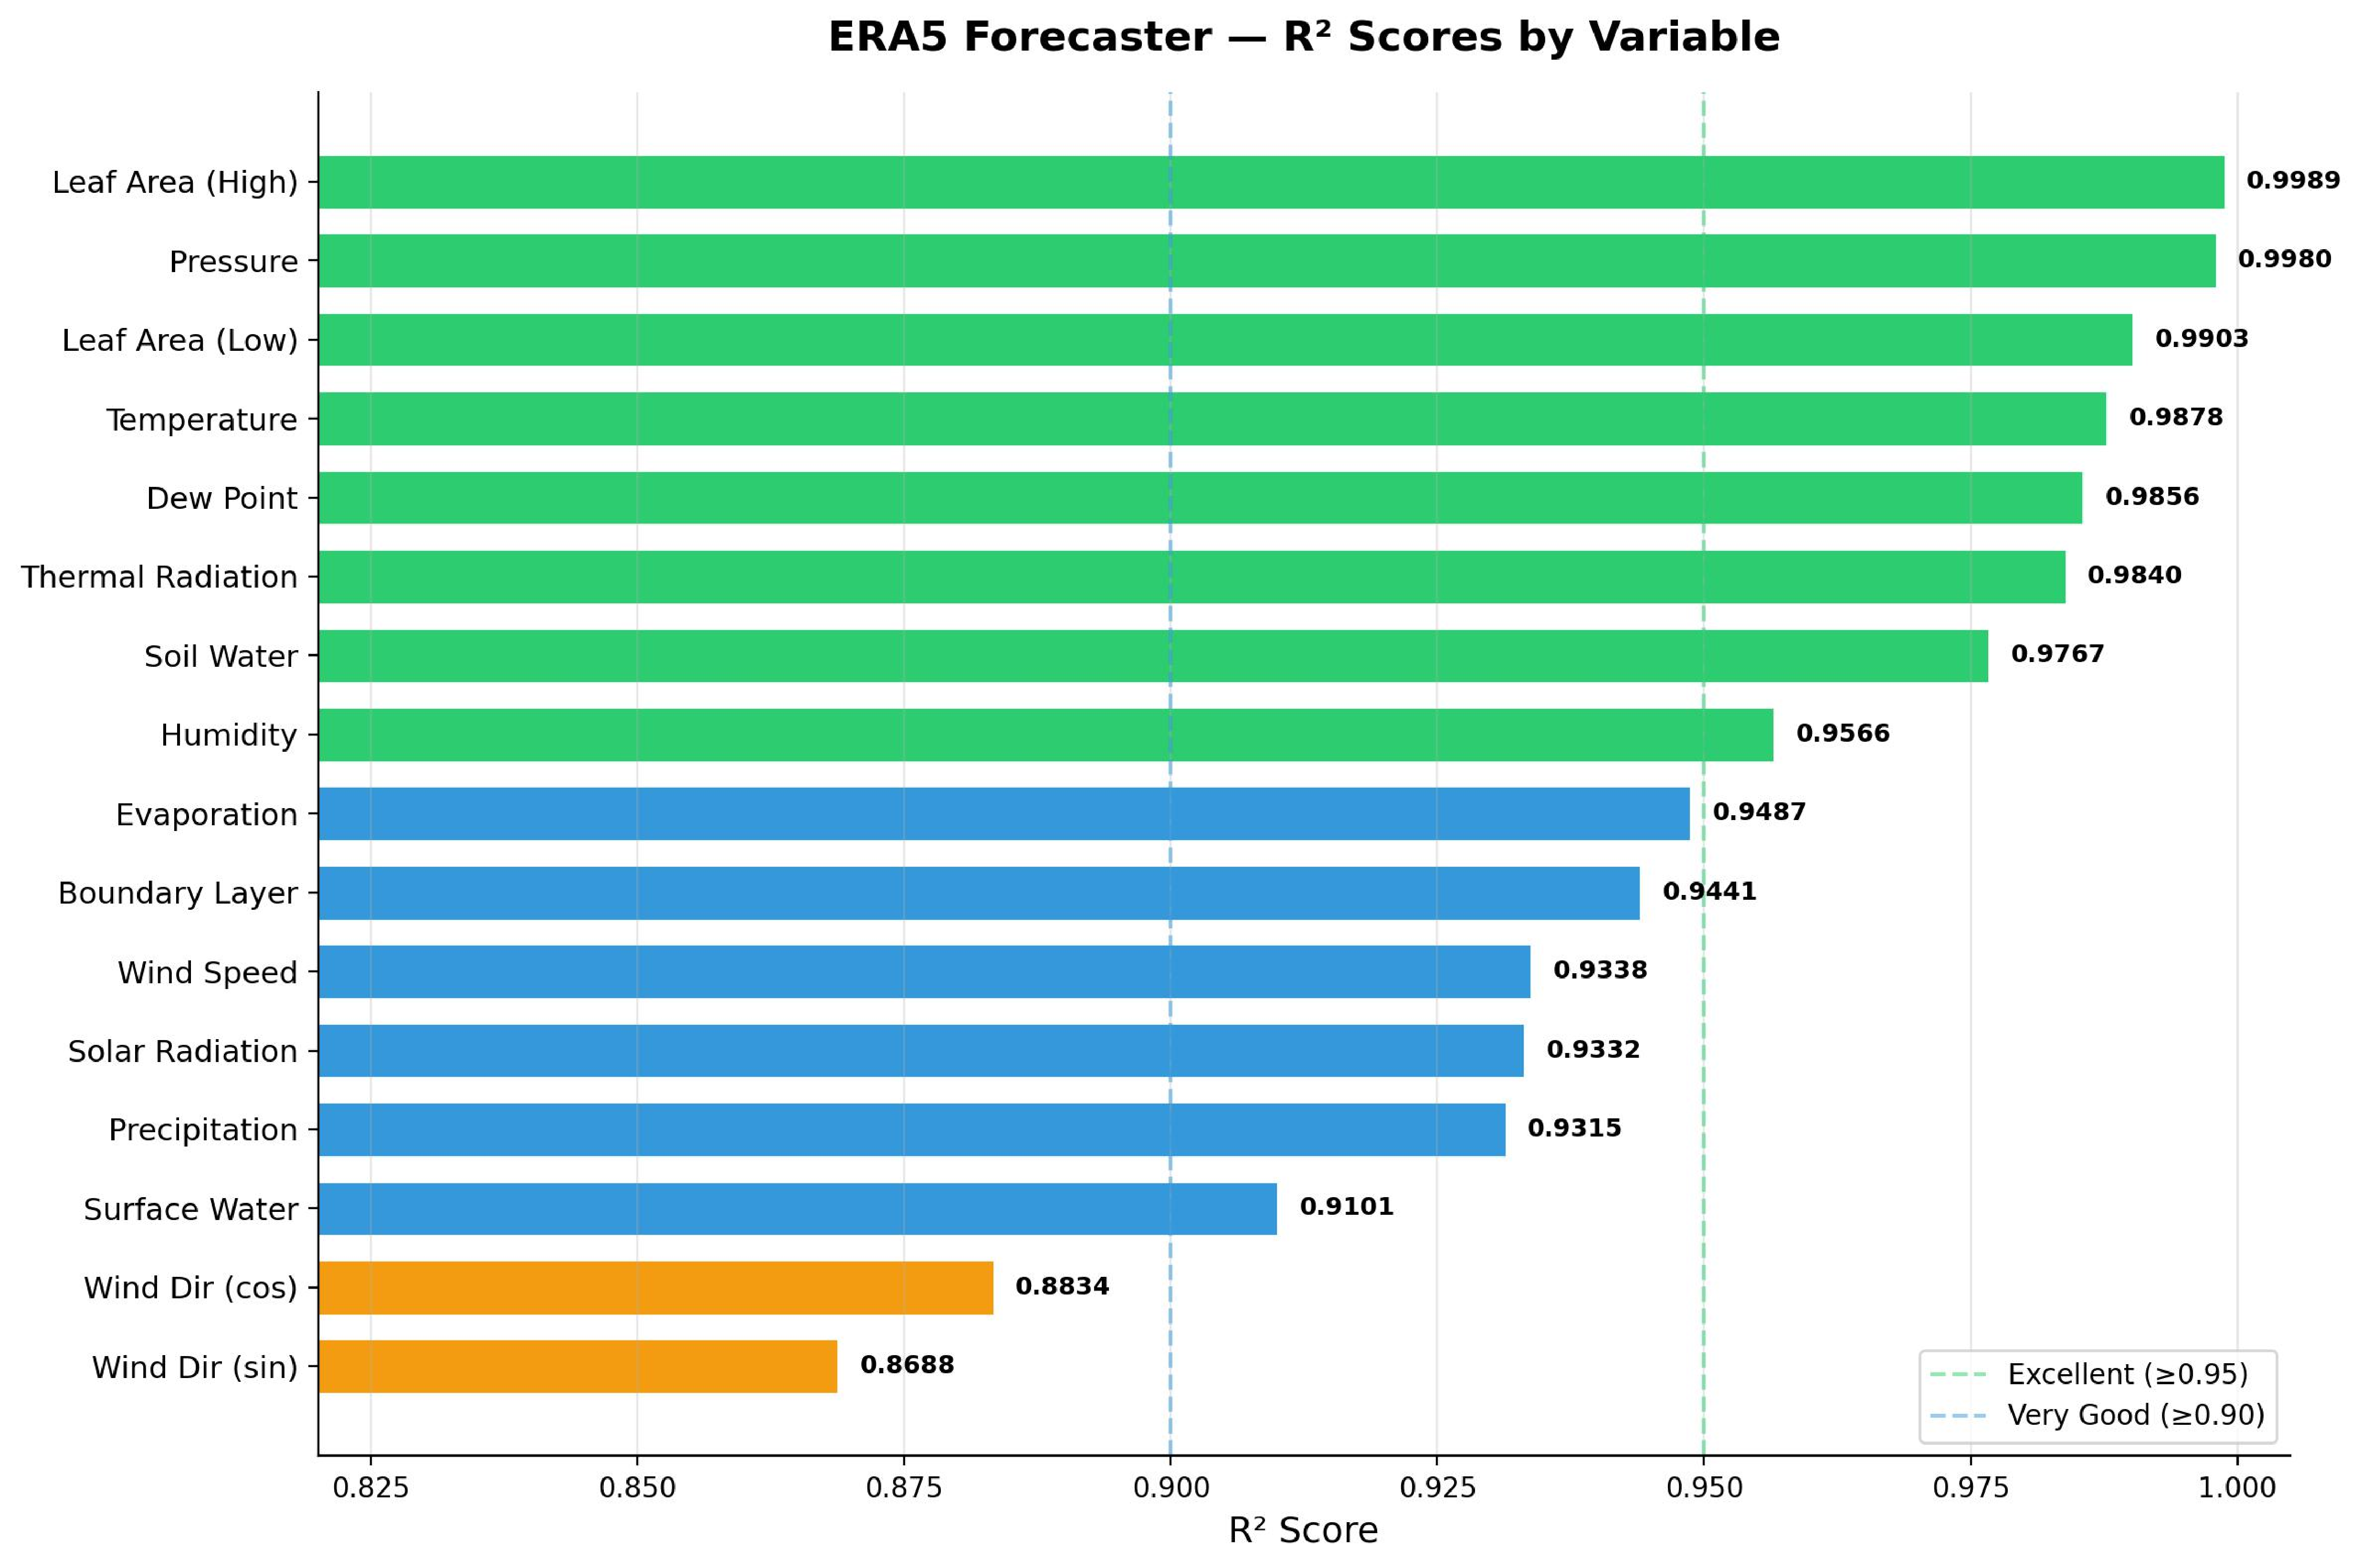
\includegraphics[width=1\linewidth]{pdfs/era5-r2.pdf} \caption{ERA-5 Forecaster $R^2$ Chart} \label{fig:placeholder} \end{figure}

\begin{figure}[H]
    \centering
    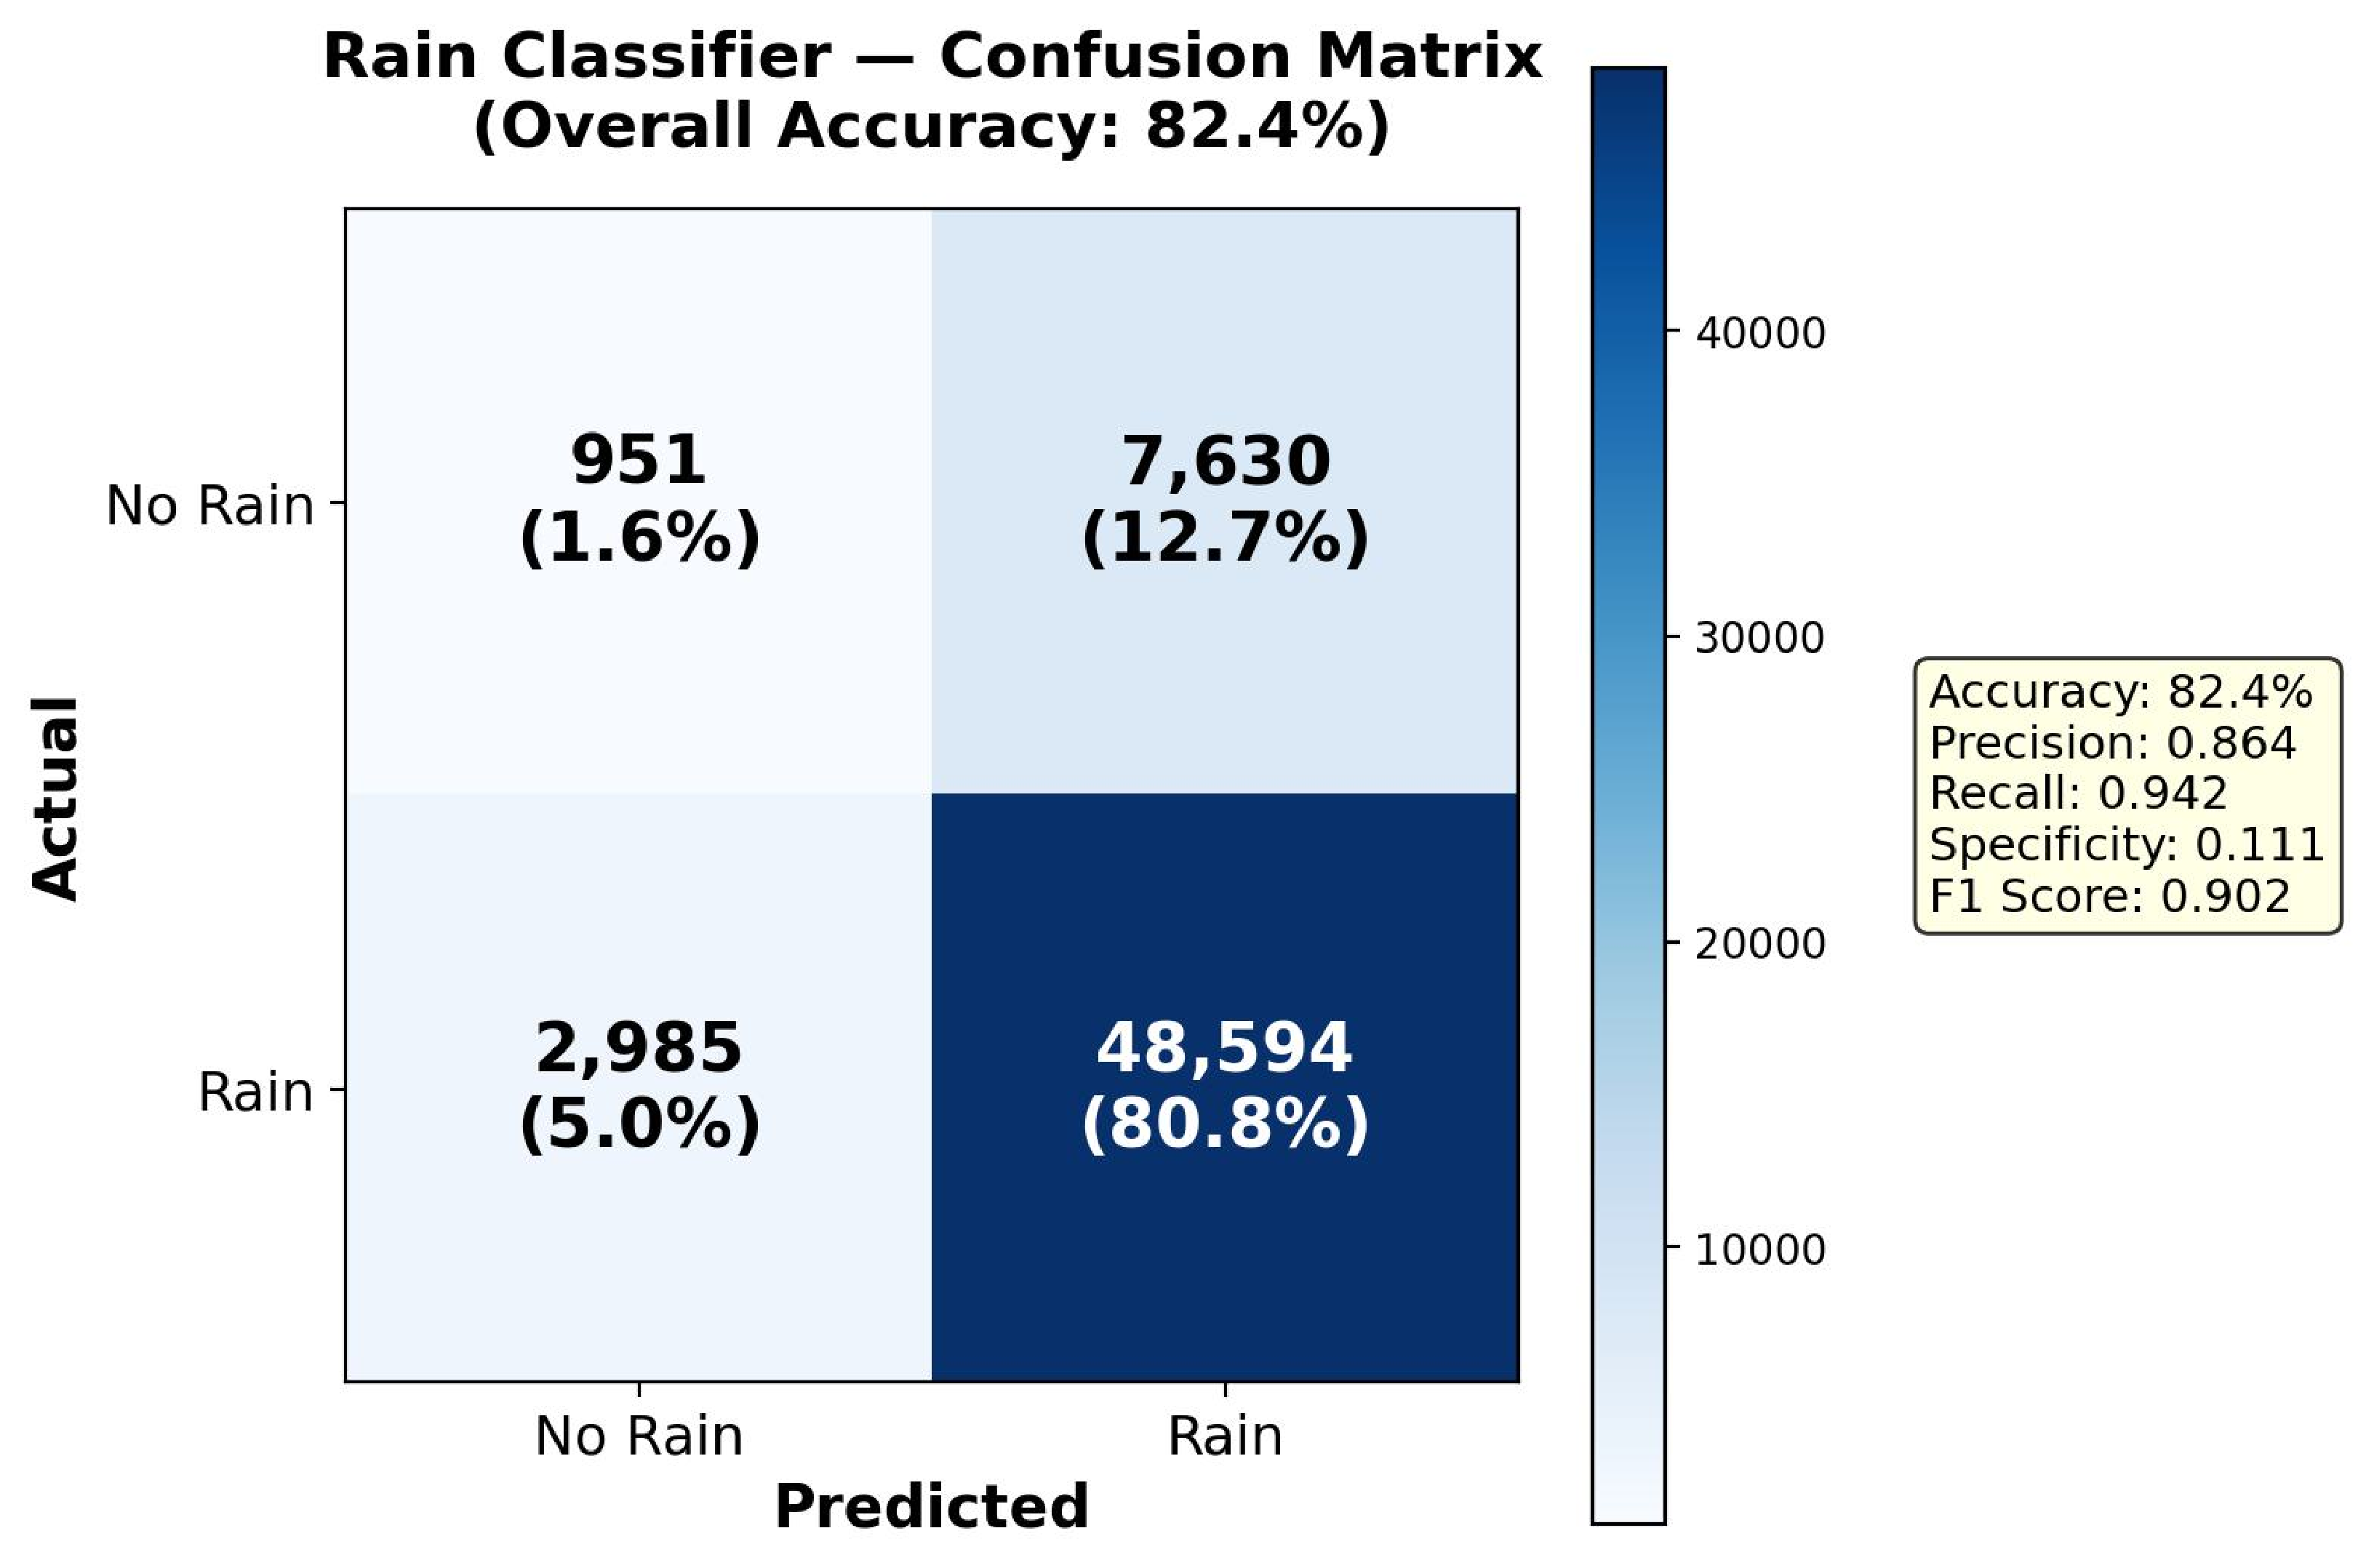
\includegraphics[width=1\linewidth]{pdfs/era5-matrix.pdf}
    \caption{ERA-5 XGBoost rain classifier}
    \label{rain_performance}
\end{figure}

\section{MODIS AOD$_{550}$ Gap-Filling and Real Time Model}

MODIS AOD$_{550}$ observations often have large gaps due to cloud cover, high aerosol variability, and satellite limitations. To create a continuous, gap-free dataset suitable for real-time PM$_{2.5}$ modeling, we implemented a machine learning-based gap-filling framework using ERA5 meteorological variables and climatology features.

\subsection{Training Sites}

At the training sites, models were trained using ERA5 variables combined with climatology features that provide day-of-year statistics to capture seasonal AOD cycles. A random split of the historical data ensured the model learned from diverse weather conditions.

\begin{table}[h!]
\centering
\caption{MODIS AOD$_{550}$ gap-filling performance at training sites.}
\label{tab:modis_training}
\vspace{.3cm}
\begin{tabular}{|l|c|c|c|c|}
\hline
\textbf{Site} & \textbf{XGB $R^2$} & \textbf{LGB $R^2$} & \textbf{Ensemble} $R^2$ & \textbf{Best Model} \\
\hline
site\_a & 0.665 & 0.655 & 0.666 & Ensemble \\
\hline
site\_b & 0.616 & 0.626 & 0.626 & Ensemble \\
\hline
site\_c & 0.709 & 0.668 & 0.695 & XGBoost \\
\hline
site\_d & 0.581 & 0.592 & 0.594 & Ensemble \\
\hline
site\_e & 0.690 & 0.695 & 0.699 & Ensemble \\
\hline
india\_a & 0.454 & 0.477 & 0.485 & Ensemble \\
\hline
india\_b & 0.475 & 0.486 & 0.489 & Ensemble \\
\hline
india\_c & 0.526 & 0.502 & 0.521 & XGBoost \\
\hline
\multicolumn{5}{|l|}{\textbf{Average  : Nepal = 0.656,  
India = 0.498}} \\
\hline
\end{tabular}
\end{table}

\subsection{Deployment Sites}

For deployment sites, a chronological split was applied to mimic real-time forecasting conditions. Two approaches were evaluated: site-specific training, using only local data, and transfer learning, leveraging models trained on multiple training sites.
\begin{enumerate}
    \item \textbf{Site-Specific:} Training and testing only on data from the deployment site.  
    \item \textbf{Transfer Learning:} Training on all training sites and then applying the learned model to the deployment site. This allows the model to leverage patterns from multiple locations, which is particularly useful when the deployment site has limited or highly variable observations.
\end{enumerate}

\begin{table}[H]
\centering
\caption{MODIS AOD$_{550}$ gap-filling performance at deployment sites.}
\label{tab:modis_deployment}
\vspace{.3cm}
\begin{tabular}{|l|c|c|c|c|c|}
\hline
\textbf{Site }     & \textbf{Site $R^2$} &\textbf{ TL $R^2$} & \textbf{Best Appr.} & \textbf{Best Model} & $\Delta R^2$ \\
\hline
Kathmandu & 0.523      & 0.660    & TL         & LightGBM       & +0.137 \\
\hline
Pokhara   & 0.590      & 0.547    & SS         & XGBoost        & −0.043 \\
\hline
Chitwan   & 0.477      & 0.506    & TL         & LightGBM       & +0.029 \\
\hline
Birgunj   & 0.380      & 0.440    & TL         & LightGBM       & +0.060 \\
\hline
\end{tabular}
\par\vspace{0.2cm}
% {\footnotesize SS = Site-Specific, TL = Transfer Learning}
\end{table}


\subsection{Result}
\begin{itemize}
\item Prediction performance at India sites and Birgunj was lower due to higher AOD variability, fewer observations, and complex terrain interactions, which created more challenging conditions for ERA5-based gap-filling.
    \item Transfer learning improved performance for 3 of 4 deployment sites by leveraging training-site patterns.  
    \item Pokhara did not benefit due to unique valley microclimate.  
    \item The final deployment model fills gaps in MODIS AOD$_{550}$ in real-time using ERA5 features when satellite data is missing.
\end{itemize}

\section{Sentinel-2 Multispectral Gap-Filling and Real Time Model}

Sentinel-2 bands often have missing observations due to clouds, snow, or sensor limitations. To produce continuous, gap-free datasets for real-time PM$_{2.5}$ modeling, all 14 spectral bands were independently predicted using ERA5 features.

\subsection{Training}

For each band:
\begin{itemize}
    \item Algorithms tested: Random Forest, XGBoost, LightGBM, CatBoost
    \item Hyperparameters optimized via 50 Optuna trials per algorithm
    \item 5-fold time series cross-validation for robust evaluation
    \item Top 30 features selected per band using Random Forest importance
\end{itemize}

\subsection{Results per Band}
\begin{table}[H]
\centering
\caption{Prediction performance for each Sentinel-2 band.}
\label{tab:s2_band_r2}
\vspace{.3cm}
\begin{tabular}{|l|c|c|l|}
\hline
\textbf{Band} & \textbf{Best Model} & \textbf{R$^2$} & \textbf{Band Type} \\
\hline
WVP  & XGBoost  & 0.938 & Atmospheric \\
\hline
B7   & LightGBM & 0.883 & Red Edge \\
\hline
B8A  & XGBoost  & 0.881 & NIR narrow \\
\hline
B9   & LightGBM & 0.868 & Water Vapour \\
\hline
B12  & XGBoost  & 0.866 & SWIR \\
\hline
B6   & CatBoost & 0.860 & Red Edge \\
\hline
B8   & LightGBM & 0.855 & NIR \\
\hline
B11  & LightGBM & 0.807 & SWIR \\
\hline
B4   & XGBoost  & 0.777 & Red (VIS) \\
\hline
B5   & XGBoost  & 0.775 & Red Edge \\
\hline
B3   & XGBoost  & 0.668 & Green (VIS) \\
\hline
AOT  & CatBoost & 0.627 & Atmospheric \\
\hline
B2   & CatBoost & 0.556 & Blue (VIS) \\
\hline
B1   & CatBoost & 0.510 & Aerosol (VIS) \\
\hline
\multicolumn{2}{|l|}{Average R$^2$} & 0.777 & 8/14 bands ≥ 0.80 \\
\hline
\end{tabular}
\par\vspace{0.2cm}
\end{table}
The table shows the predictive performance (R$^2$) for each Sentinel-2 band using the best-performing algorithm. Higher R$^2$ indicates better gap-filling accuracy.

MODIS and Sentinel-5P training sites were used for transfer learning because their outputs exhibit strong seasonal and temporal patterns driven by regional meteorology and emissions, which can be learned and transferred to deployment locations. In contrast, Sentinel-2 provides high-resolution, location-specific surface reflectance that   is highly location-specific and lacks consistent temporal patterns across sites. Consequently, training-site-based transfer learning and gap-filling were not applied to Sentinel-2 to avoid introducing artificial spatial signals.

\subsection{Band Group Predictability}

\begin{table}[H]
\centering
\caption{Average predictability by band group.}
\label{tab:s2_band_group}
\vspace{.3cm}
\begin{tabular}{|l|c|p{8cm}|}
\hline
\textbf{Band Group} & \textbf{Avg R$^2$} & \textbf{Reason} \\
\hline
NIR + Red Edge (B5--B8A) & 0.859 & Dominated by vegetation reflectance; phenology + moisture captured by ERA5 \\
\hline
SWIR (B9, B11, B12) & 0.847 & Sensitive to soil/vegetation water content; linked to ERA5 soil moisture and precipitation \\
\hline
Visible (B1--B4) & 0.628 & Affected by atmospheric scattering; not directly captured by ERA5 \\
\hline
WVP & 0.938 & ERA5 includes humidity and dew point, directly predicts this band \\
\hline
AOT & 0.627 & Aerosol Optical Thickness not measured by ERA5; harder to predict \\
\hline
\end{tabular}
\par\vspace{0.2cm}
\end{table}
This table groups bands by type to illustrate which spectral ranges are more predictable from ERA5 features. NIR and SWIR bands perform best, while visible and aerosol-sensitive bands are less predictable.

\begin{figure}[H]
    \centering
    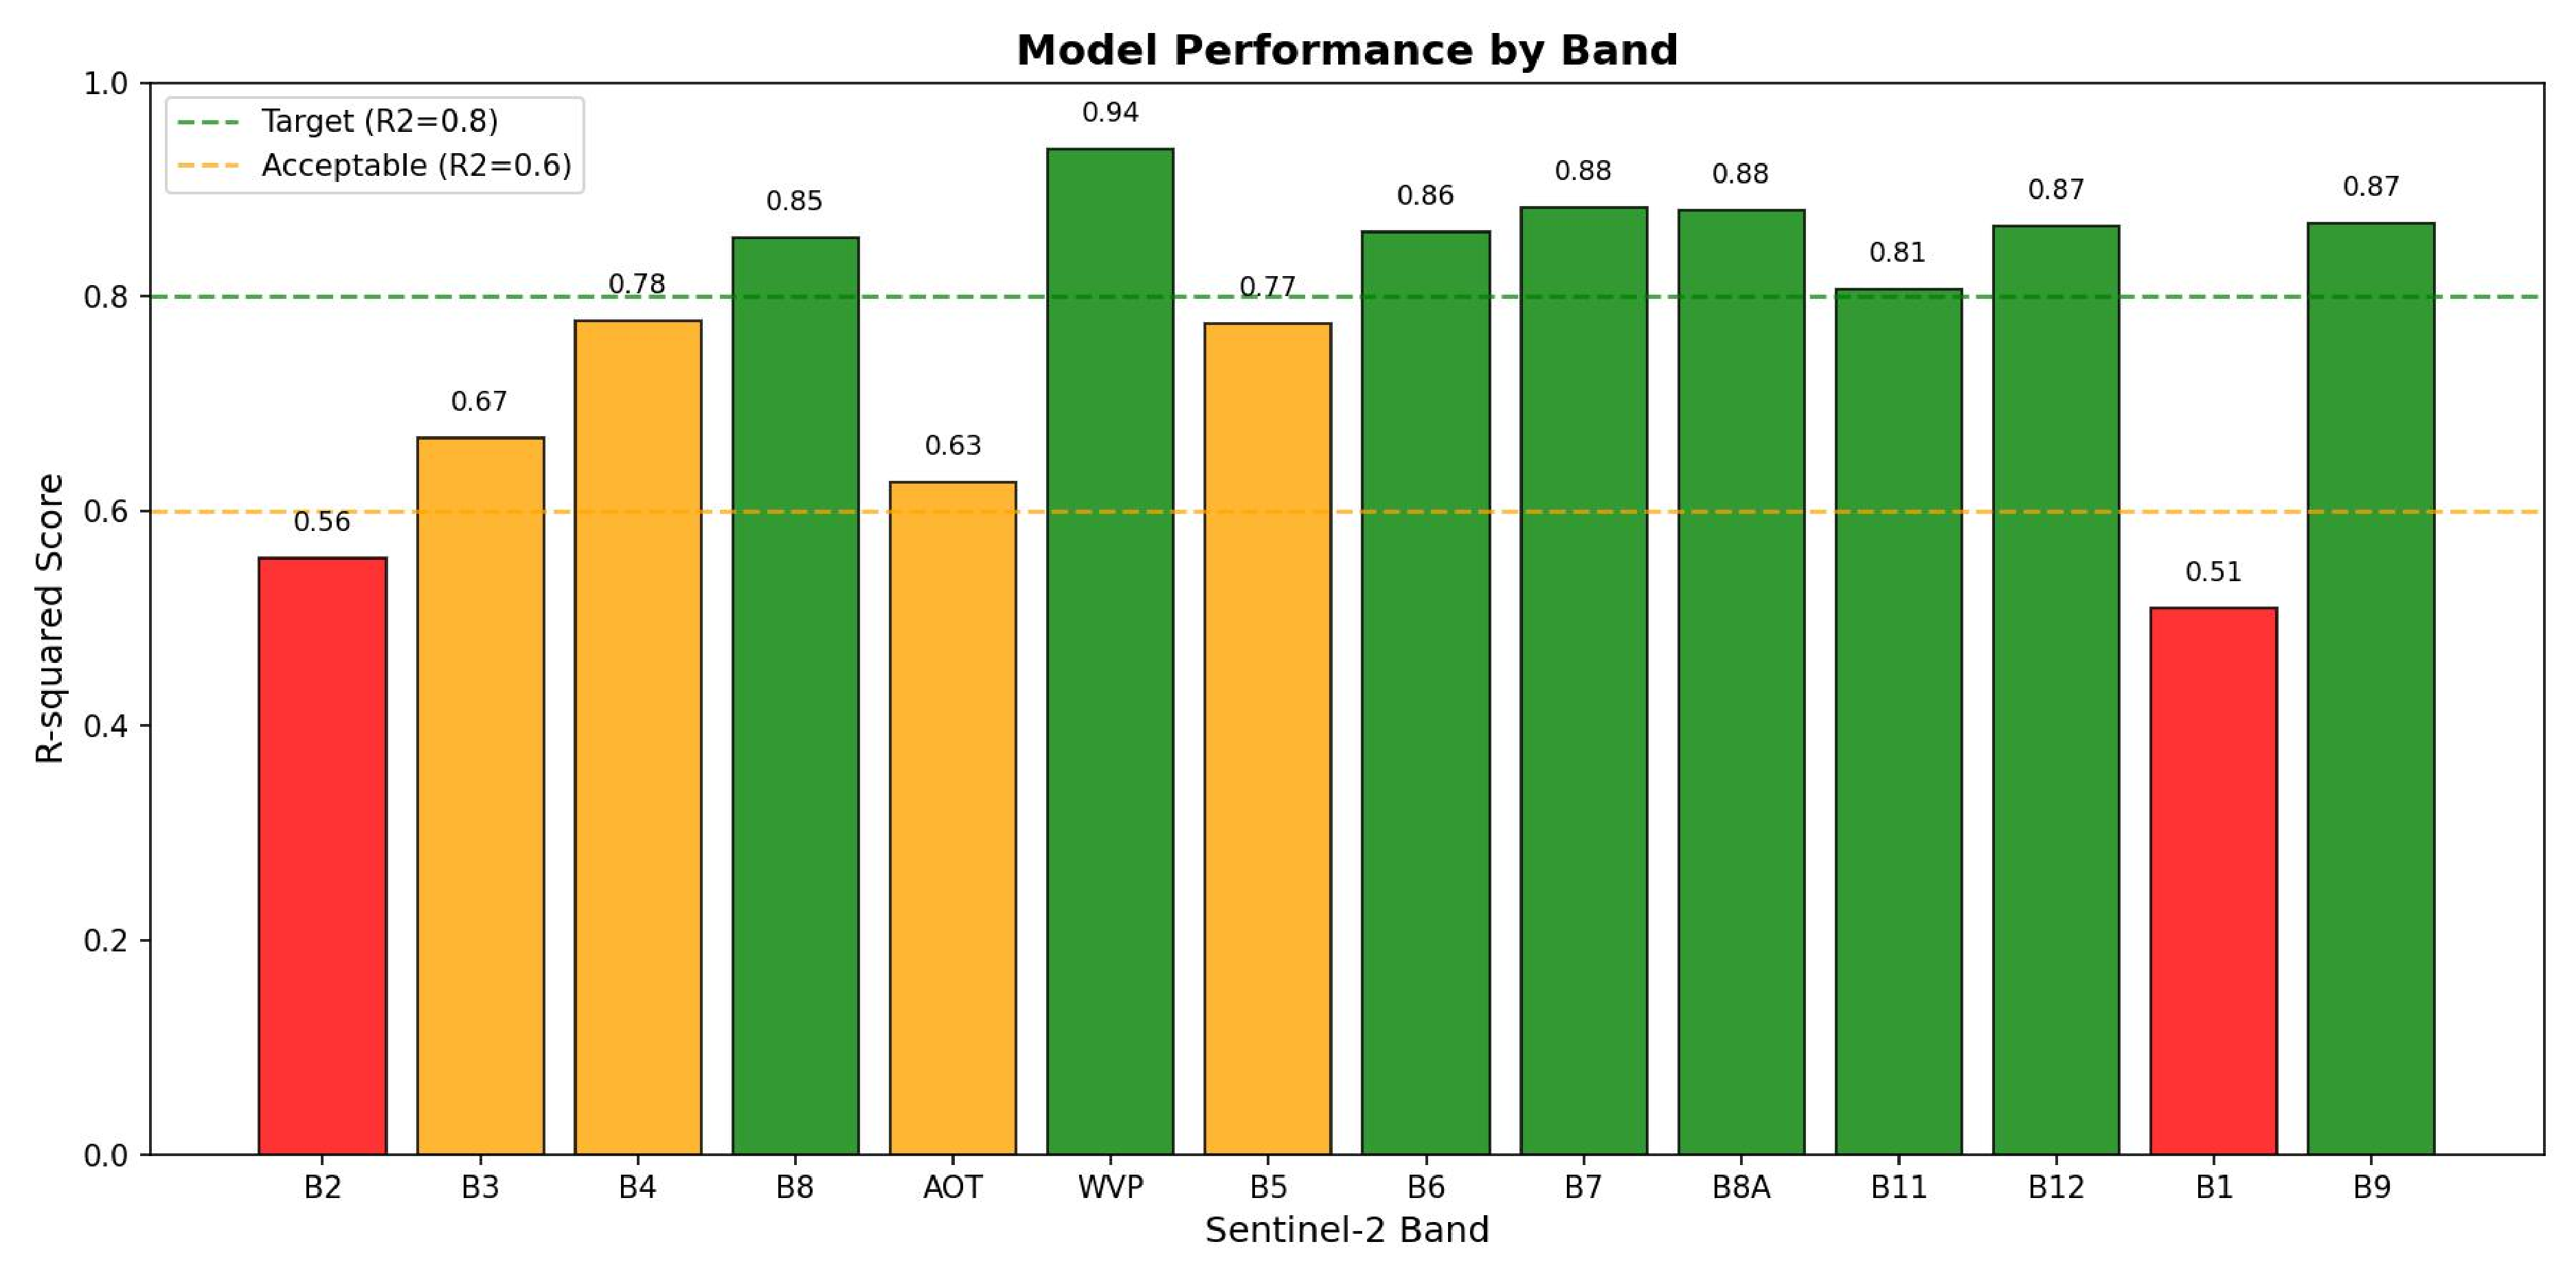
\includegraphics[width=1\linewidth]{pdfs/s2-score.pdf}
    \caption{Prediction Performance Chart}
    \label{fig:placeholder}
\end{figure}

\section{Sentinel-5P Tropospheric Gas Gap-Filling and Real Time Model}

Sentinel-5P products often have missing observations due to clouds, instrument limitations, or transient pollution events. To create continuous, gap-free datasets for real-time PM$_{2.5}$ modeling, CatBoost was used as the predictive algorithm for all features because of its superior performance in low-signal, noisy regression tasks and its ability to handle temporal features (seasonality) effectively.

\subsection{Training Site}
For the training sites, a random split of the available historical data was used to train and test temporary models to fill gaps and create a complete dataset. This allowed the models to learn general patterns of each feature without being biased by specific time periods. Table~\ref{tab:s5p_training} shows the average predictive performance of each feature.
\begin{table}[H]
\centering
\caption{Average training-site R$^2$ for Sentinel-5P features using CatBoost.}
\label{tab:s5p_training}
\vspace{.3cm}
\begin{tabular}{|l|c|p{8cm}|}
\hline
\textbf{Feature} & \textbf{Avg R$^2$} & \textbf{Notes} \\
\hline
CO   & 0.60 & Long atmospheric lifetime; large-scale seasonal and meteorological patterns captured by ERA5. \\
\hline
NO$_2$ & 0.40 & Daily average influenced by boundary layer height; ERA5 captures BLH and temperature. \\
\hline
O$_3$  & 0.50 & Photochemically produced; partly predictable from solar radiation and temperature. \\
\hline
HCHO & 0.16 & Short-lived VOC; high spatial variability not represented in ERA5. \\
\hline
AI   & 0.08 & Sensitive to absorbing aerosols; episodic events (dust, fires) not predictable from ERA5. \\
\hline
SO$_2$ & 0.04 & Point-source industrial emissions dominate; ERA5 provides no information on emissions. \\
\hline
\end{tabular}
\end{table}

Table~\ref{tab:s5p_training} show that CO, NO$_2$, and O$_3$ can be reasonably predicted using ERA5, while HCHO, AI, and SO$_2$ remain difficult due to high spatial/temporal variability or lack of meteorological control.

\subsection{Deployment Site}

For deployment sites, a chronological split was used to simulate real-time conditions, ensuring that the models only had access to past data when predicting future values. Additionally, a transfer learning approach was applied: models trained on the completed training-site dataset were adapted to each deployment site.
Table~\ref{tab:s5p_deployment} summarizes the performance of permanent models for each site.
\begin{table}[H]
\centering
\caption{Deployment-site R$^2$ for Sentinel-5P features using CatBoost.}
\label{tab:s5p_deployment}
\vspace{.3cm}
\begin{tabular}{|l|c|c|c|c|c|}
\hline
\textbf{Feature} & \textbf{Kathmandu} & \textbf{Pokhara} & \textbf{Chitwan} & \textbf{Birgunj} & \textbf{Average} \\
\hline
CO   & 0.576 & 0.662 & 0.662 & 0.502 & 0.600 \\
\hline
NO$_2$ & 0.532 & 0.423 & 0.463 & 0.171 & 0.397 \\
\hline
O$_3$  & 0.478 & 0.548 & 0.475 & 0.479 & 0.495 \\
\hline
HCHO & 0.173 & 0.098 & 0.203 & 0.178 & 0.163 \\
\hline
AI   & 0.112 & 0.322 & 0.021 & -0.134 & 0.080 \\
\hline
SO$_2$ & 0.052 & 0.046 & 0.087 & -0.027 & 0.040 \\
\hline
\end{tabular}
\end{table}
Deployment results highlight that CO and NO$_2$ remain reasonably predictable due to strong meteorological control, while SO$_2$, AI, and HCHO continue to show very low R$^2$ values. Birgunj consistently exhibits the lowest performance across all features due to trans-boundary pollution, localized industrial emissions, and complex meteorology.

\begin{figure}[H]
    \centering
    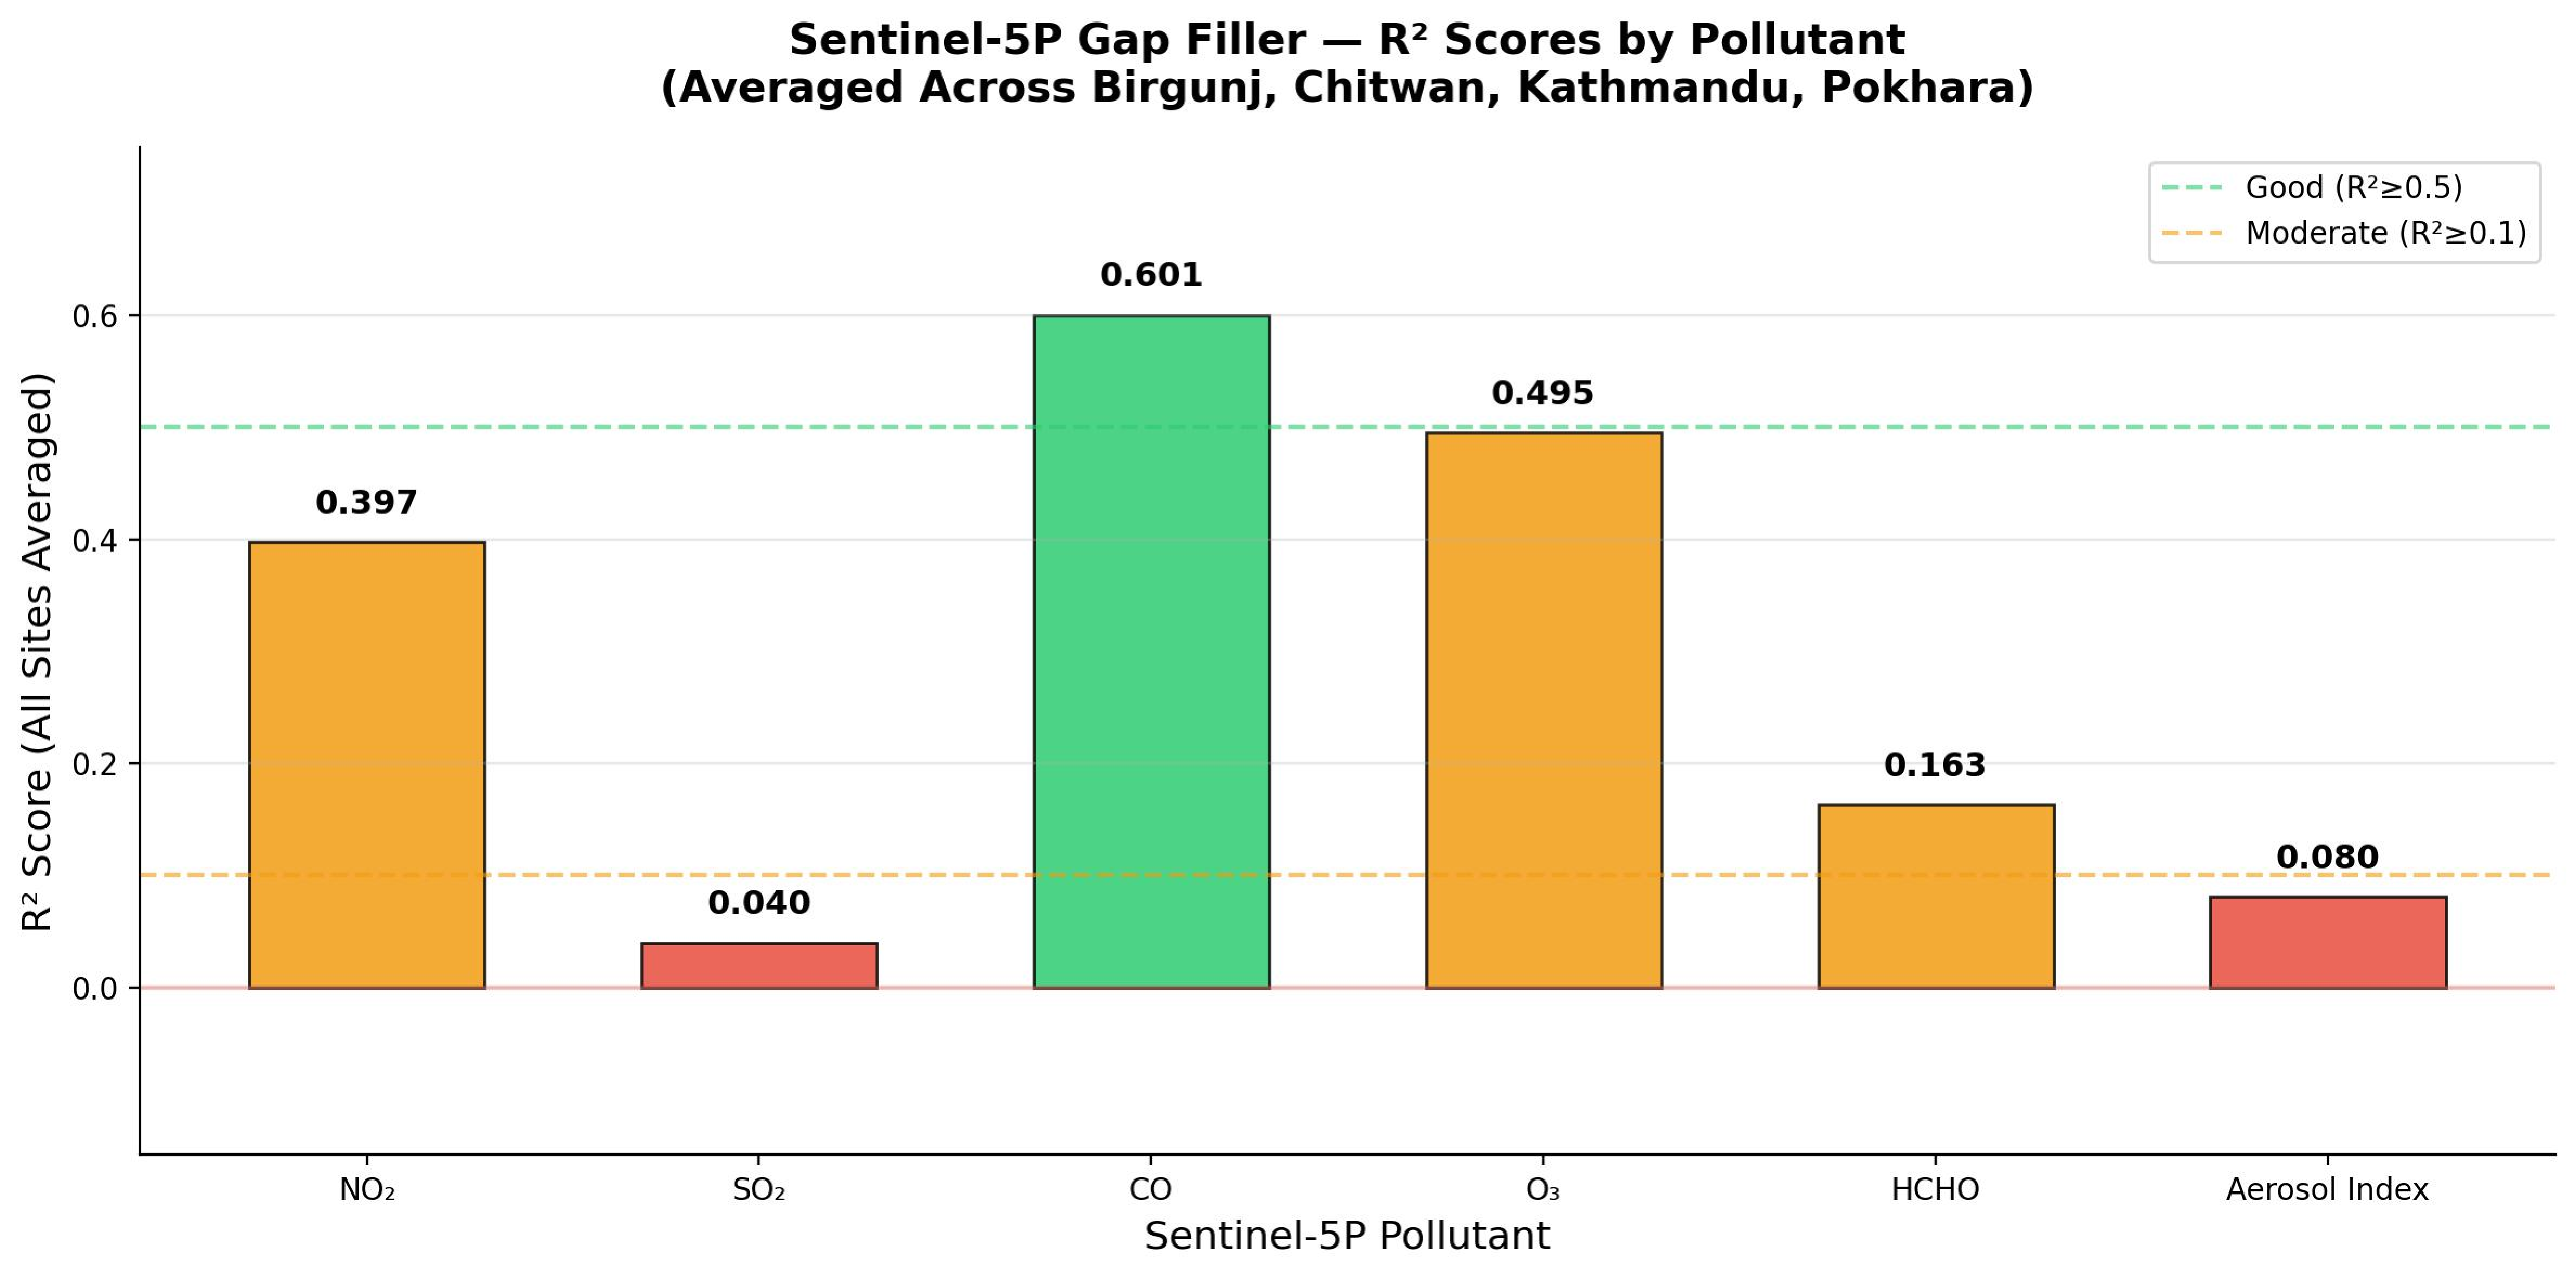
\includegraphics[width=0.75\linewidth]{pdfs/sp5-score.pdf}
    \caption{Prediction Performance Chart}
    \label{fig:placeholder}
\end{figure}

\subsection*{Practical Recommendation}

For features that remain poorly predicted (HCHO, AI, SO$_2$), these are not imputed in real time. The ensemble PM$_{2.5}$ model automatically handles missing values, relying only on authentic satellite measurements where available.

\section{Baseline PM$_{2.5}$ Modelling}

As an initial benchmark, several machine learning models were tested to predict PM$_{2.5}$ using satellite products (MODIS, Sentinel-2, Sentinel-5P) together with ERA5 meteorological variables. The models were trained using data from five Nepali training sites. Data from Indian sites were excluded to focus the baseline on local conditions. The goal of this baseline experiment was to understand the achievable performance before applying site-specific tuning or advanced modelling strategies.

All models were evaluated using a chronological 75-25 split. Model performance was assessed using R$^2$, mean absolute error (MAE), root mean square error (RMSE), and a relative accuracy metric defined as predictions within $\pm25\%$ of the observed PM$_{2.5}$ value.

The following algorithms were evaluated: Random Forest, XGBoost, LightGBM, CatBoost, and a stacking ensemble.

\begin{table}[h!]
\centering
\caption{Baseline PM$_{2.5}$ prediction performance on the test set.}
\label{tab:pm25_baseline}
\vspace{0.3cm}
\begin{tabular}{|l|c|c|c|c|}
\hline
\textbf{Model} & \textbf{R$^2$} & \textbf{MAE ($\mu$g/m$^3$)} & \textbf{RMSE ($\mu$g/m$^3$)} & \textbf{Accuracy (\%)} \\
\hline
Random Forest & 0.7616 & 10.2868 & 14.5177 & 53.46 \\
\hline
XGBoost & 0.7433 & 10.8281 & 15.0618 & 52.79 \\
\hline
LightGBM & 0.7574 & 10.4424 & 14.6427 & 51.92 \\
\hline
CatBoost & \textbf{0.7903} & \textbf{9.9042} & \textbf{13.6132} & \textbf{55.77} \\
\hline
Stacking Ensemble & 0.7827 & 9.8639 & 13.8597 & 55.29 \\
\hline
\end{tabular}
\end{table}

Overall, all models show similar performance, with R$^2$ values between 0.74 and 0.79. CatBoost performs best among the tested models, giving the highest R$^2$ and lowest error values. 

\subsection*{Model Selection Rationale}

Multiple decision tree based algorithms (Random Forest, XGBoost, LightGBM, CatBoost) were tested instead of relying on a single model. No algorithm consistently outperforms others across all targets, consistent with the \textit{No Free Lunch} theorem \citep{wolpert1996lack}, which holds that no method is universally superior across all data distributions.

The targets here (spectral bands, AOD, tropospheric gases) vary in noise, non-linearity, temporal structure, and predictability from ERA5 features. These differences align differently with each algorithm's strengths:

\begin{itemize}
    \item XGBoost excels on targets with complex interactions and moderate noise.
    \item LightGBM performs well on smoother, higher-sample signals.
    \item CatBoost handles noisier or lower-predictability targets more robustly.
\end{itemize}

Per-target selection via Optuna hyperparameter tuning and time-series cross-validation maximized gap-filling accuracy. A fixed algorithm would have underperformed on mismatched targets. This targeted approach is standard in heterogeneous remote sensing and tabular regression tasks.

\chapter{Tasks Remaining}

The successful completion of this project requires several critical components to be developed, optimized, and integrated into a cohesive real-time PM$_{2.5}$ prediction and forecasting system. The remaining tasks are organized into four major categories: model optimization and validation, LSTM forecasting model development, real-time deployment pipeline development, and system integration and testing. Each task is essential for ensuring robust performance across all deployment sites in Nepal and northern India.

\section{Model Optimization and Validation}

\subsection{Real-time Satellite Data Model Fine-tuning}

Accurate real-time satellite data predictions are foundational for the downstream PM$_{2.5}$ prediction models, as actual satellite observations (MODIS, Sentinel-2, and Sentinel-5P) are often delayed during operational deployment. Existing models require refinement to achieve the necessary predictive performance. This involves systematic evaluation to identify underperforming models, followed by retraining with optimized hyperparameters, temporal aggregation strategies, and ensemble techniques. Rigorous validation against observed satellite data is crucial to ensure that the predicted satellite values maintain sufficient accuracy for subsequent PM$_{2.5}$ estimation.

\subsection{PM$_{2.5}$ Prediction Model Enhancement}

The ensemble PM$_{2.5}$ prediction model represents the core of the same-day air quality estimation system. While baseline models for the Nepali training sites have been established, three Indian training sites currently lack reliable models due to data quality issues. Development of these models entails comprehensive data preprocessing, outlier handling, and imputation strategies to mitigate the effects of missing or noisy observations.  

Feature engineering is a critical step in enhancing model performance. Temporal features such as day-of-week, seasonality indicators, and lagged values are combined with spatial and domain-specific features derived from meteorological and satellite variables. Candidate ensemble algorithms—including Random Forest, XGBoost, LightGBM, CatBoost, and stacking ensembles—undergo hyperparameter optimization to maximize predictive accuracy. Additionally, transfer learning approaches are explored to leverage patterns learned from high-quality Nepali sites for improving predictions at Indian sites.  

Finally, a systematic evaluation determines whether unified models suffice or region-specific models are necessary. Correlation analysis and performance assessment guide the decision, ensuring that final models are specifically tuned for the four deployment sites, which represent the ultimate operational environment.

\section{LSTM-based Forecasting Model Development}

The Long Short-Term Memory (LSTM) network provides 7-day PM$_{2.5}$ forecasts by capturing temporal dependencies in historical patterns. The model processes sequences of 45 days, integrating multi-dimensional inputs that include historical satellite data, meteorological variables, and ensemble model PM$_{2.5}$ predictions. Designing the LSTM architecture involves selecting the optimal number of layers, hidden units, dropout rates, and activation functions to balance model complexity with forecasting accuracy.  

Training and validation are performed using temporally ordered datasets to prevent information leakage, and performance is evaluated across multiple forecast horizons. Special attention is given to the storage and retrieval of ensemble model predictions, ensuring seamless integration between the real-time prediction and LSTM forecasting components. Region-specific variations are considered if separate ensemble models are deployed, allowing for flexible LSTM architectures that accommodate different site characteristics.

\section{Real-time Deployment Pipeline Development}

Developing a robust end-to-end pipeline is critical for operational deployment. The pipeline automates the execution of satellite data prediction models, feature engineering, PM$_{2.5}$ estimation, and storage of results for LSTM forecasting. This includes:

\begin{itemize}
    \item Automated acquisition and prediction of satellite parameters for all deployment sites.
    \item Integration of real-time meteorological data and construction of derived features.
    \item Feeding engineered inputs into trained ensemble PM$_{2.5}$ models and storing outputs in a structured database.
    \item Execution of the LSTM forecasting pipeline using the continuously updated 45-day rolling dataset.
    \item Implementation of monitoring, error handling, and logging mechanisms to ensure reliability and detect anomalies during production operation.
\end{itemize}

The pipeline ensures that all components operate in a coordinated manner, providing consistent and accurate real-time predictions and forecasts for end users.

\section{System Integration and Testing}

The final stage of the project involves integrating all developed components and validating the complete system. End-to-end testing is conducted across all deployment sites, comparing predictions and forecasts against ground truth measurements from OpenAQ. Performance evaluation includes metrics for both same-day PM$_{2.5}$ predictions and multi-day forecasts, ensuring that the models and pipelines function cohesively in operational conditions. Comprehensive documentation of system architecture, data flows, and operational procedures is prepared to facilitate maintenance, future updates, and reproducibility of results.






\addcontentsline{toc}{section}{References}
\renewcommand{\bibname}{References}
\bibliographystyle{unsrt}
\bibliography{ref}
\end{document}
